\begin{filecontents*}{references.bib}
@inproceedings{agarwal2021,
  author    = {Agarwal, Rishabh and Schwarzer, Max and Castro, Pablo Samuel and Courville, Aaron C. and Bellemare, Marc G.},
  title     = {Deep reinforcement learning at the edge of the statistical precipice},
  booktitle = {Advances in Neural Information Processing Systems},
  volume    = {34},
  pages     = {29304--29320},
  year      = {2021},
  url       = {https://arxiv.org/abs/2108.13264},
  urldate   = {2026-09-05}
}

@inproceedings{amershi2019,
  author    = {Amershi, Saleema and Weld, Daniel and Vorvoreanu, Mihaela and Fourney, Adam and Nushi, Besmira and Collisson, Penny and others},
  title     = {Guidelines for human-{AI} interaction},
  booktitle = {Proceedings of the 2019 CHI Conference on Human Factors in Computing Systems},
  pages     = {1--13},
  year      = {2019},
  doi       = {10.1145/3290605.3300233}
}

@incollection{basili1994,
  author    = {Basili, Victor R. and Caldiera, Gianluigi and Rombach, H. Dieter},
  title     = {Goal question metric approach},
  booktitle = {Encyclopedia of Software Engineering},
  editor    = {Marciniak, John J.},
  publisher = {John Wiley \& Sons},
  location  = {New York},
  pages     = {528--532},
  year      = {1994}
}

@article{cardamone2010,
  author  = {Cardamone, Luigi and Loiacono, Daniele and Lanzi, Pier Luca},
  title   = {Learning to drive in the {Open Racing Car Simulator} using online neuroevolution},
  journal = {IEEE Transactions on Computational Intelligence and AI in Games},
  volume  = {2},
  number  = {3},
  pages   = {176--190},
  year    = {2010},
  doi     = {10.1109/TCIAIG.2010.2052102}
}

@inproceedings{fujimoto2018,
  author    = {Fujimoto, Scott and van Hoof, Herke and Meger, David},
  title     = {Addressing function approximation error in actor-critic methods},
  booktitle = {Proceedings of the 35th International Conference on Machine Learning},
  volume    = {80},
  pages     = {1587--1596},
  year      = {2018},
  url       = {https://proceedings.mlr.press/v80/fujimoto18a.html},
  urldate   = {2026-09-05}
}

@article{guidotti2019,
  author  = {Guidotti, Riccardo and Monreale, Anna and Ruggieri, Salvatore and Turini, Franco and Giannotti, Fosca and Pedreschi, Dino},
  title   = {A survey of methods for explaining black box models},
  journal = {ACM Computing Surveys},
  volume  = {51},
  number  = {5},
  pages   = {93},
  year    = {2019},
  doi     = {10.1145/3236009}
}

@article{hevner2004,
  author  = {Hevner, Alan R. and March, Salvatore T. and Park, Jinsoo and Ram, Sudha},
  title   = {Design science in information systems research},
  journal = {MIS Quarterly},
  volume  = {28},
  number  = {1},
  pages   = {75--105},
  year    = {2004},
  doi     = {10.2307/25148625}
}

@inproceedings{henderson2018,
  author    = {Henderson, Peter and Islam, Riashat and Bachman, Philip and Pineau, Joelle and Precup, Doina and Meger, David},
  title     = {Deep reinforcement learning that matters},
  booktitle = {Proceedings of the AAAI Conference on Artificial Intelligence},
  volume    = {32},
  number    = {1},
  year      = {2018},
  doi       = {10.1609/aaai.v32i1.11694}
}

@article{hohman2019,
  author  = {Hohman, Fred and Kahng, Minsuk and Pienta, Robert and Chau, Duen Horng},
  title   = {Visual analytics in deep learning: An interrogative survey for the next frontiers},
  journal = {IEEE Transactions on Visualization and Computer Graphics},
  volume  = {25},
  number  = {8},
  pages   = {2674--2693},
  year    = {2019},
  doi     = {10.1109/TVCG.2018.2843369}
}

@online{iso29148,
  author  = {{ISO/IEC/IEEE}},
  title   = {{ISO/IEC/IEEE 29148:2018 Systems and software engineering: Life cycle processes: Requirements engineering}},
  year    = {2018},
  location = {Geneva},
  url     = {https://www.iso.org/standard/72089.html},
  urldate = {2026-09-05}
}

@inproceedings{lillicrap2016,
  author    = {Lillicrap, Timothy P. and Hunt, Jonathan J. and Pritzel, Alexander and Heess, Nicolas and Erez, Tom and Tassa, Yuval and others},
  title     = {Continuous control with deep reinforcement learning},
  booktitle = {International Conference on Learning Representations},
  year      = {2016},
  url       = {https://arxiv.org/abs/1509.02971},
  urldate   = {2026-09-05}
}

@inproceedings{long2020,
  author    = {Long, Duri and Magerko, Brian},
  title     = {What is {AI} literacy? Competencies and design considerations},
  booktitle = {Proceedings of the 2020 CHI Conference on Human Factors in Computing Systems},
  pages     = {1--16},
  publisher = {Association for Computing Machinery},
  year      = {2020},
  doi       = {10.1145/3313831.3376727}
}

@article{loiacono2010,
  author  = {Loiacono, Daniele and Lanzi, Pier Luca and Togelius, Julian and Onieva, Enrique and Pelta, David A. and Butz, Martin V. and others},
  title   = {The 2009 simulated car racing championship},
  journal = {IEEE Transactions on Computational Intelligence and AI in Games},
  volume  = {2},
  number  = {2},
  pages   = {131--147},
  year    = {2010},
  doi     = {10.1109/TCIAIG.2010.2050590}
}

@online{nielsen1994,
  author  = {Nielsen, Jakob},
  title   = {10 usability heuristics for user interface design},
  organization = {Nielsen Norman Group},
  year    = {1994},
  url     = {https://www.nngroup.com/articles/ten-usability-heuristics/},
  urldate = {2026-09-05}
}

@inproceedings{onieva2009,
  author    = {Onieva, Enrique and Pelta, David A. and Alonso, Jos{\'e} and Milan{\'e}s, Vicente and P{\'e}rez, Jorge},
  title     = {A modular parametric architecture for the {TORCS} racing engine},
  booktitle = {2009 IEEE Symposium on Computational Intelligence and Games},
  pages     = {256--262},
  year      = {2009},
  doi       = {10.1109/CIG.2009.5286466}
}

@article{peffers2007,
  author  = {Peffers, Ken and Tuunanen, Tuure and Rothenberger, Marcus A. and Chatterjee, Samir},
  title   = {A design science research methodology for information systems research},
  journal = {Journal of Management Information Systems},
  volume  = {24},
  number  = {3},
  pages   = {45--77},
  year    = {2007},
  doi     = {10.2753/MIS0742-1222240302}
}

@inproceedings{quadflieg2010,
  author    = {Quadflieg, Jan and Preuss, Mike and Kr{\"a}mer, Oliver and Rudolph, G{\"u}nter},
  title     = {Learning the track and planning ahead in a car racing controller},
  booktitle = {2010 IEEE Conference on Computational Intelligence and Games},
  pages     = {395--402},
  year      = {2010},
  doi       = {10.1109/ITW.2010.5593327}
}

@inproceedings{ribeiro2016,
  author    = {Ribeiro, Marco Tulio and Singh, Sameer and Guestrin, Carlos},
  title     = {Why should I trust you?: Explaining the predictions of any classifier},
  booktitle = {Proceedings of the 22nd ACM SIGKDD International Conference on Knowledge Discovery and Data Mining},
  pages     = {1135--1144},
  year      = {2016},
  doi       = {10.1145/2939672.2939778}
}

@book{russellnorvig2021,
  author    = {Russell, Stuart J. and Norvig, Peter},
  title     = {Artificial Intelligence: A Modern Approach},
  edition   = {4},
  publisher = {Pearson},
  location  = {Hoboken, NJ},
  year      = {2021}
}

@inproceedings{sutton1990,
  author    = {Sutton, Richard S.},
  title     = {Integrated architectures for learning, planning, and reacting based on approximating dynamic programming},
  booktitle = {Proceedings of the Seventh International Conference on Machine Learning},
  pages     = {216--224},
  year      = {1990},
  doi       = {10.1016/B978-1-55860-141-3.50030-4}
}

@book{suttonbarto2018,
  author    = {Sutton, Richard S. and Barto, Andrew G.},
  title     = {Reinforcement Learning: An Introduction},
  edition   = {2},
  publisher = {MIT Press},
  location  = {Cambridge, MA},
  year      = {2018}
}

@online{torcs2026,
  author  = {{TORCS}},
  title   = {{TORCS}: The Open Racing Car Simulator},
  year    = {2026},
  url     = {https://sourceforge.net/projects/torcs/},
  urldate = {2026-09-05}
}

@article{watkinsdayan1992,
  author  = {Watkins, Christopher J. C. H. and Dayan, Peter},
  title   = {Q-learning},
  journal = {Machine Learning},
  volume  = {8},
  number  = {3--4},
  pages   = {279--292},
  year    = {1992},
  doi     = {10.1007/BF00992698}
}

@online{wcag22,
  author  = {{World Wide Web Consortium}},
  title   = {Web Content Accessibility Guidelines ({WCAG}) 2.2},
  year    = {2024},
  url     = {https://www.w3.org/TR/WCAG22/},
  urldate = {2026-09-05}
}

\end{filecontents*}

% MAT099 dissertation manuscript
% Compile with: pdflatex main && biber main && pdflatex main && pdflatex main
\documentclass[12pt,a4paper]{article}

\usepackage[T1]{fontenc}
\usepackage[utf8]{inputenc}
\usepackage{lmodern}
\usepackage{microtype}
\usepackage[a4paper,margin=25mm]{geometry}
\usepackage{setspace}
\usepackage{graphicx}
\usepackage{booktabs}
\usepackage{tabularx}
\usepackage{array}
\usepackage{amsmath}
\usepackage{enumitem}
\usepackage{csquotes}
\usepackage{titlesec}
\usepackage{hyperref}
\usepackage[nameinlink,noabbrev]{cleveref}
\usepackage[backend=biber,style=authoryear,sorting=nyt,maxcitenames=3,mincitenames=1,giveninits=true]{biblatex}

\addbibresource{references.bib}
\graphicspath{{figures/}}
\onehalfspacing
\setlength{\emergencystretch}{3em}
\setlist{nosep}
\newcolumntype{Y}{>{\raggedright\arraybackslash}X}
\setcounter{secnumdepth}{2}
\setcounter{tocdepth}{2}
\numberwithin{figure}{section}
\numberwithin{table}{section}
\titleformat{\section}
  {\normalfont\Large\bfseries}
  {\thesection}
  {0.75em}
  {}
\titlespacing*{\section}{0pt}{3.25ex plus 1ex minus .2ex}{1.25ex plus .2ex}
\titleformat{\subsection}
  {\normalfont\large\bfseries}
  {\thesubsection}
  {0.75em}
  {}
\titlespacing*{\subsection}{0pt}{2.5ex plus .8ex minus .2ex}{0.9ex plus .2ex}
\hypersetup{
  colorlinks=true,
  linkcolor=black,
  citecolor=black,
  urlcolor=blue,
  pdftitle={Enhanced AI Racing},
  pdfauthor={Nathaniel Bassett}
}

\newcommand{\dissertationtitle}{Enhanced AI Racing: A Novice-Friendly Platform for Evaluating Autonomous Driving Agents in TORCS}
\newcommand{\authorname}{Nathaniel Bassett}
\newcommand{\studentnumber}{21087358}
\newcommand{\degreeprogramme}{MSc Data Science and Analytics}
\newcommand{\supervisorname}{Dr Nico Potoyka}

\begin{document}

\begin{titlepage}
\centering
\thispagestyle{empty}

\vspace*{1.2cm}


\includegraphics[height=3.1cm]{CU_Logo.jpg}\par

\vspace{2.2cm}

{\Large\bfseries
Enhanced AI Racing: A\par
\vspace{0.18cm}
Novice-Friendly Platform for\par
\vspace{0.18cm}
Evaluating Autonomous Driving\par
\vspace{0.18cm}
Agents in TORCS\par
}

\vspace{2.4cm}

{\large Nathaniel Bassett\par}

\vspace{2.4cm}

{\large September 2026\par}

\vspace{1.7cm}

{\large School of Mathematics,\par}
{\large Cardiff University\par}

\vfill

\begin{minipage}{0.72\textwidth}
\centering
\small
A dissertation submitted in partial fulfilment of the\\
requirements for the degree of MSc Data Science and Analytics,\\
supervised by Dr Nico Potoyka.
\end{minipage}

\end{titlepage}

\pagenumbering{roman}

\section*{Declaration}
\addcontentsline{toc}{section}{Declaration}
% Replace this text with the University-approved declaration from the MAT099 template.
\noindent [Insert the University-approved declaration here.]

\section*{Acknowledgements}
\addcontentsline{toc}{section}{Acknowledgements}
% Intentionally left for the author.
\noindent [Acknowledgements to be completed by the author.]

\section*{Executive Summary}
\addcontentsline{toc}{section}{Executive Summary}

Enhanced AI Racing is an individual MSc dissertation project that develops and evaluates autonomous racing agents in the TORCS simulator. Its purpose is not only to make an artificial intelligence driver complete a circuit. It is also to make the behaviour of different AI approaches understandable to people who are new to artificial intelligence, reinforcement learning and software development. The project responds directly to the brief's requirement for a novice-friendly launcher and wrapper around the TORCS racing environment.

The problem has two sides. Autonomous racing is technically difficult because a driver must repeatedly decide how to steer, accelerate and brake while remaining on the track. A very fast action can cause the car to spin, leave the circuit or fail to complete a lap. A useful evaluation must therefore consider both pace and reliability. At the same time, many AI projects are difficult for beginners to access: they require installation of software packages, command-line setup and interpretation of technical logs before any behaviour can be observed. Enhanced AI Racing addresses these issues in one application by combining driving agents, telemetry capture, persistent results, visual comparison and a packaged Windows release.

The project implements a progression of autonomous-control approaches: a random baseline, a rule-based anti-spin driver, a map-aware racing-line driver, a Dyna-Q learner and two deep reinforcement-learning agents based on N-step Twin Delayed Deep Deterministic Policy Gradients (TD3). The sequence makes it possible to compare explicit control logic, track knowledge and learned continuous control rather than treating one final neural policy as the only meaningful outcome.

The TD3 agents provide the most informative learned comparison. Agent~7 uses racing-line geometry as context, while Agent~8 uses vehicle telemetry, track-edge sensors and short-term driving history without reading a racing-line file or receiving external teacher actions. Agent~8's final stability profile uses self-imitation from its own successful trajectories. This tests whether a sensor-only policy can learn competitive behaviour while retaining a transparent distinction between the agents' information sources and training histories.

All reported races use the \texttt{g-track-3} circuit, the same car and a one-lap task. The system records completion, completed-lap time, off-track behaviour, stalling, reverse driving and timeouts as telemetry and persistent run data. Completion rate is always reported with its number of attempts; median completed-lap time represents typical successful pace; and failures remain visible.

The hand-engineered map-aware controller is a strong benchmark: it completed all 15 stored application runs and achieved a 92.056-second median completed lap. The rule-based agent was slower but stable. Dyna-Q completed only one of three stored runs, and early scratch TD3 produced no completed stored lap. These outcomes show that reinforcement learning was not assumed to be successful simply because it was more technically advanced.

The strongest final learned result came from Agent~8. Across two repeated 20-run evaluation batches, Agent~8 completed 36 of 40 attempts, a 90\% completion rate, with a median completed-lap time of 83.038 seconds. Agent~7 also achieved reliable learned behaviour: one final policy completed 18 of 20 attempts, while a later policy completed 10 of 10 in a smaller batch, but its completed laps were slower. The results therefore suggest that, for the implemented policies and the selected circuit, Agent~8 achieved the strongest observed combination of pace and repeated completion. They do not prove that sensor-only learning is always better than racing-line information, nor that the policy would transfer unchanged to other tracks or real vehicles.

The application is a second major result. Users can extract the release folder and start \texttt{EnhancedAIRacing.exe} without creating a Python environment or configuring TORCS manually. The interface supports agent selection, live telemetry, saved-run review, comparison and plain-language agent explanations. A packaged-release smoke test verifies that the dashboard opens, policies load, TORCS starts from the application and completed runs are stored. This provides functional evidence that the project is easier to run and inspect than a source-only research prototype.

The project is limited to simulated racing, one principal track and functional evaluation of the novice-facing interface. It does not claim road-safety performance or proven educational improvement without participant testing. Future work should evaluate final agents in equal-sized frozen-policy batches, test unseen tracks, isolate racing-line input in a controlled ablation and conduct a small novice-user study. Within scope, Enhanced AI Racing delivers a working, distributable and evidence-aware platform for studying how autonomous agents drive, fail, improve and can be explained.

\section*{Software and Artefact Availability}
\addcontentsline{toc}{section}{Software and Artefact Availability}

The source code and implementation documentation for Enhanced AI Racing are available at \url{https://github.com/natebassett/mat099-enhanced-ai-racing} (Accessed: 6 September 2026). The repository supports reproducibility and technical audit; the packaged Windows release remains the intended route for novice users.
\tableofcontents
\listoffigures
\listoftables

\clearpage
\pagenumbering{arabic}

\section{Introduction}
\label{ch:introduction}

\subsection{Context and problem}

Autonomous racing is a compact but demanding control problem. A driver must translate changing observations into continuous steering, throttle and braking actions while balancing speed against the risk of leaving the circuit. The decision is sequential: an action that appears beneficial at one instant can create an unrecoverable position or heading several seconds later. Simulation makes this problem practical for a dissertation because repeated trials can be performed without the safety, cost and reproducibility constraints of real vehicles.

TORCS provides a suitable environment because it exposes a driving task with vehicle dynamics, track geometry and sensor observations, while allowing controllers to be connected programmatically \parencite{torcs2026}. It has been used in autonomous-racing competitions and research as a repeatable testbed for computational-intelligence controllers \parencite{loiacono2010}. However, a simulator alone does not produce useful research. A project must make the chosen agents comparable, preserve the evidence from their runs and distinguish a genuinely reliable policy from an isolated successful lap.

There is a second, practical problem. AI racing projects often require users to install a simulator, configure a Python environment, locate model files and interpret raw logs before they can observe any behaviour. That route is reasonable for developers but unsuitable for a novice learner. The MAT099 brief therefore requires not only a functioning AI driver, but a user-friendly launcher and beginner-facing wrapper that makes the system engaging and consumable. This dissertation treats that requirement as an engineering and research concern, rather than as a cosmetic interface layer.

Enhanced AI Racing addresses both problems. It provides several controller families in one application, records their telemetry and outcomes, and presents the information through an interface designed for running, reviewing and comparing races. The work does not claim to solve real-world autonomous driving. Its scope is simulated autonomous racing in TORCS and the communication of that behaviour to users who do not need to read the implementation to begin learning from it.

\subsection{Aim, questions and objectives}

The aim was to design, implement and evaluate a TORCS-based AI racing platform that compares autonomous driving approaches and presents their behaviour through a research-informed desktop learning platform for adult and university-level newcomers to artificial intelligence.

The dissertation answers four questions:
\begin{enumerate}[label=\arabic*.]
  \item How can rule-based, map-aware and reinforcement-learning agents be implemented within one shared TORCS application?
  \item Under a common racing scenario, how do the agents differ in completion, pace and failure behaviour?
  \item How can a packaged interface use telemetry, results provenance and explanation design to help an AI newcomer launch, observe and critically compare those differences without source-level setup?
  \item What limitations arise from using one simulator, one principal circuit and a resource-constrained development process?
\end{enumerate}

The objectives were to build a reliable runner between Python and TORCS; implement a ladder of increasingly capable agents; store telemetry and race outcomes; create a graphical interface and distributable Windows package; and evaluate the agents with a protocol that reports failures as well as successful laps. The project is an individual dissertation. All implementation, agent design, experiments and application integration reported here were undertaken by the author.

\subsection{Contributions and dissertation structure}

The principal contribution is not a claim that one policy is a universal racing solution. It is a coherent research and learning artefact. Technically, it supplies multiple control paradigms behind a common action contract, including a final comparison between racing-line-informed and sensor-only N-step Twin Delayed Deep Deterministic Policy Gradient (TD3). As software, it couples simulation control to SQLite-backed telemetry, results review and a packaged executable. As a research-informed learning platform, it is designed to expose the distinction between a rule, a policy, a reward and an evaluation outcome through visible racing consequences; it does not claim validated learning outcomes without a participant study.

The contribution also lies in the relationship between these parts. The graphical wrapper is not described as a separate demonstration added after the technical work. It consumes the same run records and evaluation summaries used in the analysis, so a chart seen by a novice and a claim made in the results chapter can be traced to the same underlying evidence. Likewise, the packaged executable is not merely a convenience for a marker; it is the route by which the project becomes usable outside the author's development environment. This integration is central to the brief's enterprise-AI and school-facing motivation.

\Cref{ch:research-context} establishes the relevant technical background. \Cref{ch:literature-review} critically relates the design to prior racing, reinforcement-learning and human-AI interaction research. Sections~4 to~6 explain the research method, requirements and architecture. Sections~7 and~8 describe the agents and the novice-facing interface. Sections~9 and~10 present the evaluation protocol and results. Sections~11 and~12 interpret the evidence, identify limitations and conclude the work.

\section{Research Context and Technical Background}
\label{ch:research-context}

\subsection{Autonomous control in TORCS}

An intelligent agent observes its environment, selects actions and pursues an objective through the consequences of those actions \parencite{russellnorvig2021}. In this project, TORCS is the environment and a Python driver is the agent. At each simulation step the driver receives observations such as speed, heading angle, track position and range-sensor readings. It returns a control action comprising steering, longitudinal control and gear selection. A racing episode is therefore a closed loop rather than a set of independent predictions.

The quality of that loop cannot be represented by speed alone. A high speed on a straight may coexist with poor heading control, repeated excursions beyond the track boundary or an incomplete lap. Conversely, a conservative controller can be slower but provide a more robust and interpretable baseline. This motivates the use of completion rate, completed-lap time, termination reason and telemetry traces as complementary measures rather than collapsing performance into a single score.

The same reasoning applies to the relationship between training and evaluation. During training, an agent may use exploratory action noise, update its parameters and occasionally encounter an unusually favourable trajectory. Evaluation must instead freeze the policy and report whether the observed behaviour can be reproduced. This distinction is particularly important in deep reinforcement learning, where a successful training episode is useful evidence of capability but not sufficient evidence of a stable deployable policy. The project preserves both forms of evidence, but uses them for different claims.

\subsection{Control approaches}

The project spans three broad approaches. Rule-based control encodes human decisions explicitly, for example reducing throttle when heading error rises or applying recovery logic during a spin. It is transparent and cheap to evaluate, but cannot react well to cases not anticipated by its rules. Map-aware control adds a representation of the route ahead. A racing line turns track knowledge into target position and curvature information, allowing a controller to prepare for a corner instead of only responding once it is already misaligned.

Reinforcement learning takes a different route. It learns a policy from interaction and a reward signal rather than specifying each driving decision directly \parencite{suttonbarto2018}. Dyna-Q combines value learning with model-based planning \parencite{sutton1990}, making it a useful bridge between tabular reinforcement learning and the simulator. TD3 is a deep actor-critic method designed for continuous control and uses twin critics, delayed policy updates and target-policy smoothing to reduce overestimation error \parencite{fujimoto2018}. Its action space is a natural fit for steering and longitudinal control, but its performance depends strongly on the observation design, reward, training experience and evaluation process.

\subsection{Explainability and novice access}

Explainability in this project does not mean claiming that a neural network can fully explain each internal feature interaction. It means giving a user sufficient evidence to form an appropriate understanding of what happened and why. Telemetry can show speed, position, control outputs and failures; comparison views can show that a fast lap is not necessarily a reliable policy; and agent descriptions can link visible behaviour to the relevant control method. This approach is consistent with human-AI interaction guidance that emphasises communicating system capability, state and limitations to users \parencite{amershi2019}.

The installation path is part of that access. A novice cannot inspect an AI system that they cannot start. The project consequently packages the dashboard, runtime dependencies, TORCS, final policies and evidence files into a Windows application folder. Users extract the release folder and run \texttt{EnhancedAIRacing.exe} rather than constructing a development environment. This is evidence of reduced deployment friction; it is not, by itself, proof that every novice understands reinforcement learning. That stronger educational claim is considered as a limitation later in the dissertation.

\section{Literature Review and Design Rationale}
\label{ch:literature-review}

This chapter does not treat prior work as a catalogue of algorithms. It identifies what existing research establishes, the assumptions it makes, and how those assumptions informed the design of Enhanced AI Racing. The review consequently links controller literature to the agent progression, reinforcement-learning literature to the evaluation protocol, and human-AI interaction literature to the novice-facing application.

\subsection{TORCS as a comparative research environment}

The Simulated Car Racing Championship showed that TORCS can provide a common interface through which controllers with different internal methods are evaluated \parencite{loiacono2010}. \textcite{cardamone2010} further demonstrated that learning-based controllers can operate in the environment. These studies establish TORCS as a useful setting for repeatable autonomous-racing experiments; they do not establish that a controller is easy to train, robust across tracks or suitable for real vehicles. Competition-style reporting can also overemphasise a best score when a research report needs to state trial conditions, failures and uncertainty.

The present project adopts TORCS for controlled comparison rather than road-autonomy validation. Its vehicle dynamics make the task meaningfully sequential: a poor action can cause later instability, not merely a local prediction error. However, one simulator and one circuit cannot represent changing weather, traffic, sensor degradation or safety-critical consequences. This limitation motivates a deliberately narrow claim: the results concern implemented policies on \texttt{g-track-3}, not real-world driving capability.

\subsection{Engineered control, planning and their assumptions}

\textcite{onieva2009} describe a modular TORCS controller in which driving behaviour is divided into steering, speed and recovery components. This supports the rule-based anti-spin agent as a substantive baseline rather than a deliberately weak comparison. Explicit rules make the cause of an action inspectable and permit targeted recovery behaviour, but they depend on cases anticipated by the developer. Good performance therefore demonstrates effective engineering under known conditions, not automatic adaptation to unplanned circumstances.

\textcite{quadflieg2010} show why learning the track and planning ahead can improve racing control. A driver that knows the route can prepare its position and speed before a corner instead of reacting only after heading error occurs. The limitation is equally important: the value of such planning depends on a reliable track representation and may not transfer to an unseen circuit without new mapping work. This trade-off directly motivates the Map-Aware Racing-Line Agent and Agent~7, which use racing-line geometry, and Agent~8, which intentionally receives no route information.

\subsection{From Dyna-Q to continuous deep reinforcement learning}

Q-learning estimates the value of taking an action in a state and provides a principled basis for learning through reward \parencite{watkinsdayan1992}. Dyna extends that idea by combining direct experience with planning updates from a learned model \parencite{sutton1990}. Dyna-Q was consequently appropriate as a bounded learning experiment: it tests whether planning can improve sample efficiency when live TORCS interaction is slow. Its likely weakness is structural rather than incidental. Continuous driving state must be discretised into bins, and a finite action set cannot express every small steering or throttle correction. The Dyna-Q agent therefore tests a useful research question without being expected to match a continuous high-performance policy.

Continuous control provides the rationale for deep actor-critic methods. Deep Deterministic Policy Gradient (DDPG) demonstrated deterministic policy learning for continuous actions \parencite{lillicrap2016}, while TD3 addresses a known weakness of actor-critic value estimation through twin critics, delayed policy updates and target-policy smoothing \parencite{fujimoto2018}. These features justify N-step TD3 for steering and longitudinal control, but they do not guarantee reliable racing. The final outcome depends on the observation contract, reward, training distribution, checkpoint selection and evaluation procedure. A policy can exploit an incomplete reward or produce a rare fast lap that is unsuitable for deployment.

This literature informed two design decisions. First, Agent~7 and Agent~8 share the TD3 foundation but retain distinct, documented observation and reward contracts. Agent~7 receives racing-line geometry as context; Agent~8 receives vehicle state, 19 track-edge sensors and short-term history, with geometry slots fixed to zero. Secondly, the final Agent~8 selection process prioritised completion rate before median completed-lap time. Its self-imitation stage used trajectories generated by Agent~8 itself, not teacher actions from an engineered driver. This is an evidence-led response to rare successful laps, but it also means that Agent~7 versus Agent~8 is not a pure one-variable ablation of racing-line information.

\subsection{Reliable evidence for learned control}

\textcite{henderson2018} show that deep-reinforcement-learning results are sensitive to implementation and evaluation choices, while \textcite{agarwal2021} argue against conclusions based only on unstable point estimates. For this project, the methodological consequence is that fastest lap is a capability measure, not a reliability measure. Completion rate must retain failed attempts in the denominator, and completed-lap pace must be reported with trial count and source.

The application therefore distinguishes integrated GUI race records from fixed-policy repeated evaluations. Both use the same core \texttt{g-track-3}, car and one-lap scenario, but their sample sizes and provenance differ. Database records demonstrate the integrated system and its stored evidence; repeated evaluation batches are stronger support for claims about final learned-policy reliability. This distinction is not a weakness to conceal. It is the information required for a reader to decide how much weight each result deserves.

\subsection{Explainability, novice access and the research gap}

Post-hoc explanation research commonly examines how to make a model prediction understandable \parencite{ribeiro2016,guidotti2019}. In a sequential control task, users also need temporal evidence: what the car observed, which action it issued, what happened next and whether it completed the lap. Visual-analytics research supports the use of interactive views for interrogating learning systems, provided that the presentation does not conceal instability or uncertainty \parencite{hohman2019}.

AI-literacy research adds a broader educational rationale. \textcite{long2020} identify competencies and design considerations that help non-specialists reason about what an AI system can do, how it operates and where its limits lie. The relevant aim here is not to teach a learner to derive TD3 or implement a neural network from first principles. It is to make the relationship between information, action, outcome and uncertainty available for inspection. Autonomous racing offers a useful setting because those relationships have immediate visible consequences: a poor steering action, an unsafe trajectory or a completed lap can be connected to recorded evidence.

The GUI applies this principle through live telemetry, stored-run review, side-by-side comparison, sample counts, failure outcomes and plain-language agent descriptions. \textcite{nielsen1994}'s visibility-of-system-status principle and \textcite{amershi2019}'s human-AI interaction guidance support this approach, particularly the choice to separate a simple novice overview from a detailed research-evidence view. The packaged executable addresses a related but distinct barrier: a learner should not need to configure Python, TORCS and policy paths before seeing an agent drive.

The resulting research gap is therefore precise. Prior work establishes that controllers can race in TORCS and that learning methods can produce continuous policies. It does not generally combine contrasting controller designs, transparent evidence provenance, a distributable novice workflow and explanation of reliability rather than only peak performance. Enhanced AI Racing addresses that gap through one artefact designed to support initial AI literacy. It does not claim to prove educational outcomes without participant testing, or to establish a universal ranking of racing algorithms.

\subsection{Literature synthesis}

\begin{table}[htbp]
  \centering
  \caption{Literature synthesis and its design implications.}
  \label{tab:literature-synthesis}
  \small
  \begin{tabularx}{\textwidth}{p{0.19\textwidth}YYY}
    \toprule
    Literature area & What it establishes & Important limitation & Design response in this project \\
    \midrule
    TORCS competition research & A common simulator can compare autonomous controllers & Strong lap results do not establish road validity or reliability & One-track claims are explicitly scoped; failures and trial counts are retained \\
    Modular and map-aware control & Explicit rules and route information can improve control & Rules depend on anticipated cases; racing lines are track-specific & Rule-Based and Map-Aware agents provide interpretable baselines \\
    Dyna-Q and TD3 & Learning can improve control; TD3 suits continuous actions & Representation, reward and evaluation can dominate the result & Dyna-Q is treated as a bounded experiment; TD3 contracts and checkpoints are preserved \\
    Human-AI interaction and XAI & Users need visible state, capability and limitations & Explanations can hide uncertainty or overwhelm novices & Progressive disclosure, telemetry, provenance and packaged access \\
    \bottomrule
  \end{tabularx}
\end{table}

\section{Research Design and Methodology}
\label{ch:methodology}

\subsection{Research strategy}

The project used an applied design-science strategy. Design science is appropriate when knowledge is generated through creating and evaluating an artefact that addresses an identified problem \parencite{hevner2004}. \textcite{peffers2007} describe a cycle of problem identification, objectives, design, demonstration, evaluation and communication. That cycle maps closely to this dissertation: the problem was not only to drive a simulated car, but to make alternative agent designs and their evidence inspectable by novice users.

The artefact was developed iteratively. A working TORCS runner and shared agent action contract came first, because every later comparison depends on consistent communication with the simulator. Baselines then established controllable behaviour before learning methods were introduced. Telemetry storage and GUI views were developed alongside the agents rather than added after evaluation, ensuring that the same records could support technical analysis and user-facing explanation. Finally, the Windows package made the completed application available without a development installation.

The iteration was evidence-led. When a controller failed, the response was not simply to add another algorithm. The random driver first checked the action path; the rule-based controller supplied observable stabilisation behaviour; map-aware control tested whether explicit route information improved the baseline; and the learning agents were introduced only once result recording was available. For Agent~8, early high-pace but low-completion outcomes changed the training objective from pace discovery to clean repeated completion. This reasoning makes the final system a sequence of justified experiments rather than a catalogue of unrelated features.

\subsection{Evaluation logic}

The evaluation follows a Goal-Question-Metric structure: the questions concern comparative driving behaviour and novice-facing explanation, so the metrics must capture both pace and reliability \parencite{basili1994}. The technical measures are lap completion, completed-lap time, progress, off-track behaviour, termination reason and control telemetry. The user-facing measures are functional evidence that agents can be selected, run, reviewed and compared through the GUI, plus a deployment smoke test for the packaged application.

For the learning-platform contribution, evaluation asks whether the intended novice route is actually available in the delivered artefact. The defined tasks are to launch the package, select a named agent, start a run, observe plain-language state and telemetry, retrieve a saved outcome, and compare reliability with pace. These are observable acceptance conditions, not a proxy questionnaire for user satisfaction or learning gain. They allow the dissertation to evaluate functional accessibility and explanation design honestly while retaining a participant study as the appropriate method for stronger educational claims.

No human participants or personal data were used. The principal ethical issue is the accuracy of claims. TORCS results are evidence about simulated autonomous racing, not road safety. Similarly, a release package demonstrates simpler deployment, while the absence of a novice participant study limits any claim that the application has proven learning outcomes. These boundaries were retained explicitly rather than hidden behind broad claims about artificial intelligence.

The research questions are answered by two complementary evidence streams. Product evidence, including automated tests, package smoke checks, screenshots and stored GUI runs, shows that the application integrates the required features. Performance evidence, including fixed-policy evaluation files, supplies repeated trial outcomes for learned drivers. Treating these streams separately improves validity. A dashboard screenshot can demonstrate that a comparison view exists, but it cannot prove neural-policy reliability. Conversely, an evaluation record can support a completion claim, but it cannot demonstrate that a beginner can locate and interpret it through the interface.

\subsection{Requirements and success criteria}

The requirements were grouped into technical, evidential and educational categories. Technically, the application had to launch TORCS, run several agent types, record a common set of outcomes and preserve policy files. Evidentially, it had to retain failed as well as successful runs and make their provenance inspectable. Educationally, it had to provide a graphical route through the system, use readable agent explanations and reduce deployment steps through the Windows package.

This treatment follows the principle of requirements engineering that capabilities and quality constraints should be stated in a form that can later be verified \parencite{iso29148}. It is especially useful here because a novice-friendly application can otherwise be evaluated impressionistically. By defining observable requirements, such as launching from the packaged folder, presenting an outcome after a race and retaining failures in a comparison, the project can demonstrate that the wrapper has delivered the requested route into the technical work even without claiming a completed human-subjects study.

The success criterion was therefore not \enquote{produce the fastest lap}. A successful project would provide a functioning and distributable AI racing application, show meaningful differences among control approaches, and allow a non-specialist to inspect that evidence without reading source code. This definition explains why stable engineered baselines, weak learning outcomes and failed episodes remain relevant results rather than being discarded.

The requirement table is deliberately concise because detailed implementation is assessed later. Its purpose is traceability. Each requirement has an observable acceptance condition, and each condition is linked to either a system test, stored experiment output or visible application behaviour. This establishes a chain from the brief, through design decisions, to evidence. It is stronger than declaring that the software is \enquote{user friendly} or \enquote{robust} without defining what those qualities require in this project.

\section{Requirements and Success Criteria}
\label{ch:requirements}

\begin{table}[htbp]
  \centering
  \caption{Traceable functional, non-functional and evidential requirements.}
  \label{tab:requirements}
  \small
  \begin{tabularx}{\textwidth}{p{0.11\textwidth}p{0.30\textwidth}Y}
    \toprule
    ID & Requirement & Evidence of success \\
    \midrule
    FR1 & Run autonomous agents in TORCS. & The runner exchanges telemetry and control actions with TORCS and records completed and failed episodes. \\
    FR2 & Support contrasting agent types. & Random, rule-based, map-aware, Dyna-Q and TD3 agents implement the common control contract. \\
    FR3 & Preserve experimental evidence. & SQLite records runs and telemetry; evaluation files retain policy path, trial outcome and contract information. \\
    FR4 & Provide a novice-facing learning workflow. & The GUI supports agent selection, live telemetry, results review, comparison and explanatory panels. \\
    NFR1 & Reduce deployment complexity. & The Windows package starts from \texttt{EnhancedAIRacing.exe} with TORCS and required runtime data included. \\
    NFR2 & Report reliability honestly. & Trial counts and failures remain visible; completed-lap medians are not presented as all-run averages. \\
    ER1 & Make behaviour interpretable. & Telemetry, outcome labels and agent-specific explanations link visible driving behaviour to AI concepts. \\
    ER2 & Support evidence-based learning. & The interface distinguishes capability, repeatability, failure and agent information sources rather than presenting a single high score. \\
    \bottomrule
  \end{tabularx}
\end{table}

The requirements are intentionally traceable to the research questions. FR1 and FR2 enable comparison; FR3 and NFR2 make the comparison defensible; FR4, NFR1, ER1 and ER2 address the brief's novice-access and learning objective. This traceability prevents the interface from becoming a feature list detached from the stated research contribution.

For the packaged release, the acceptance condition is practical: a user should not have to install Python, activate a virtual environment, configure a TORCS path or locate a policy checkpoint before observing a race. The release folder must remain intact because the executable depends on the adjacent internal runtime. The smoke test checks the novice route from opening the dashboard through starting TORCS to locating a completed run. This is more defensible than promising universal ease of use without a testable definition.

The educational requirements also constrain results presentation. The interface must not label an agent \enquote{best} solely because it has one fast record. It must show whether the claim is based on application history or repeated evaluation, include a trial count, and retain failures in the comparison. These requirements matter because an accessible wrapper that hides uncertainty would be easier to use but educationally misleading.

The requirements also define what the application deliberately does not do. It does not train a policy from the main beginner workflow, silently alter protected runtime checkpoints, or merge evidence from different evaluations into an unexplained aggregate. These exclusions preserve a stable interface and make the result of pressing Start understandable: the user is running a named, fixed agent under a selected scenario, not triggering an opaque background experiment.

\section{System Architecture}
\label{ch:architecture}

\subsection{Architecture and data flow}

The application is organised around six responsibilities: TORCS simulation, a Python runner, agent implementations, telemetry and storage, the desktop GUI, and separate training/evaluation scripts. \Cref{fig:architecture-overview} depicts the agent-environment loop and evidence flow. TORCS provides observations; the selected agent produces steering, throttle, brake and gear decisions; the runner applies them and records the resulting state; storage persists both run-level outcomes and time-series telemetry; and the GUI reloads those records for live and post-race inspection.

\begin{figure}[htbp]
  \centering
  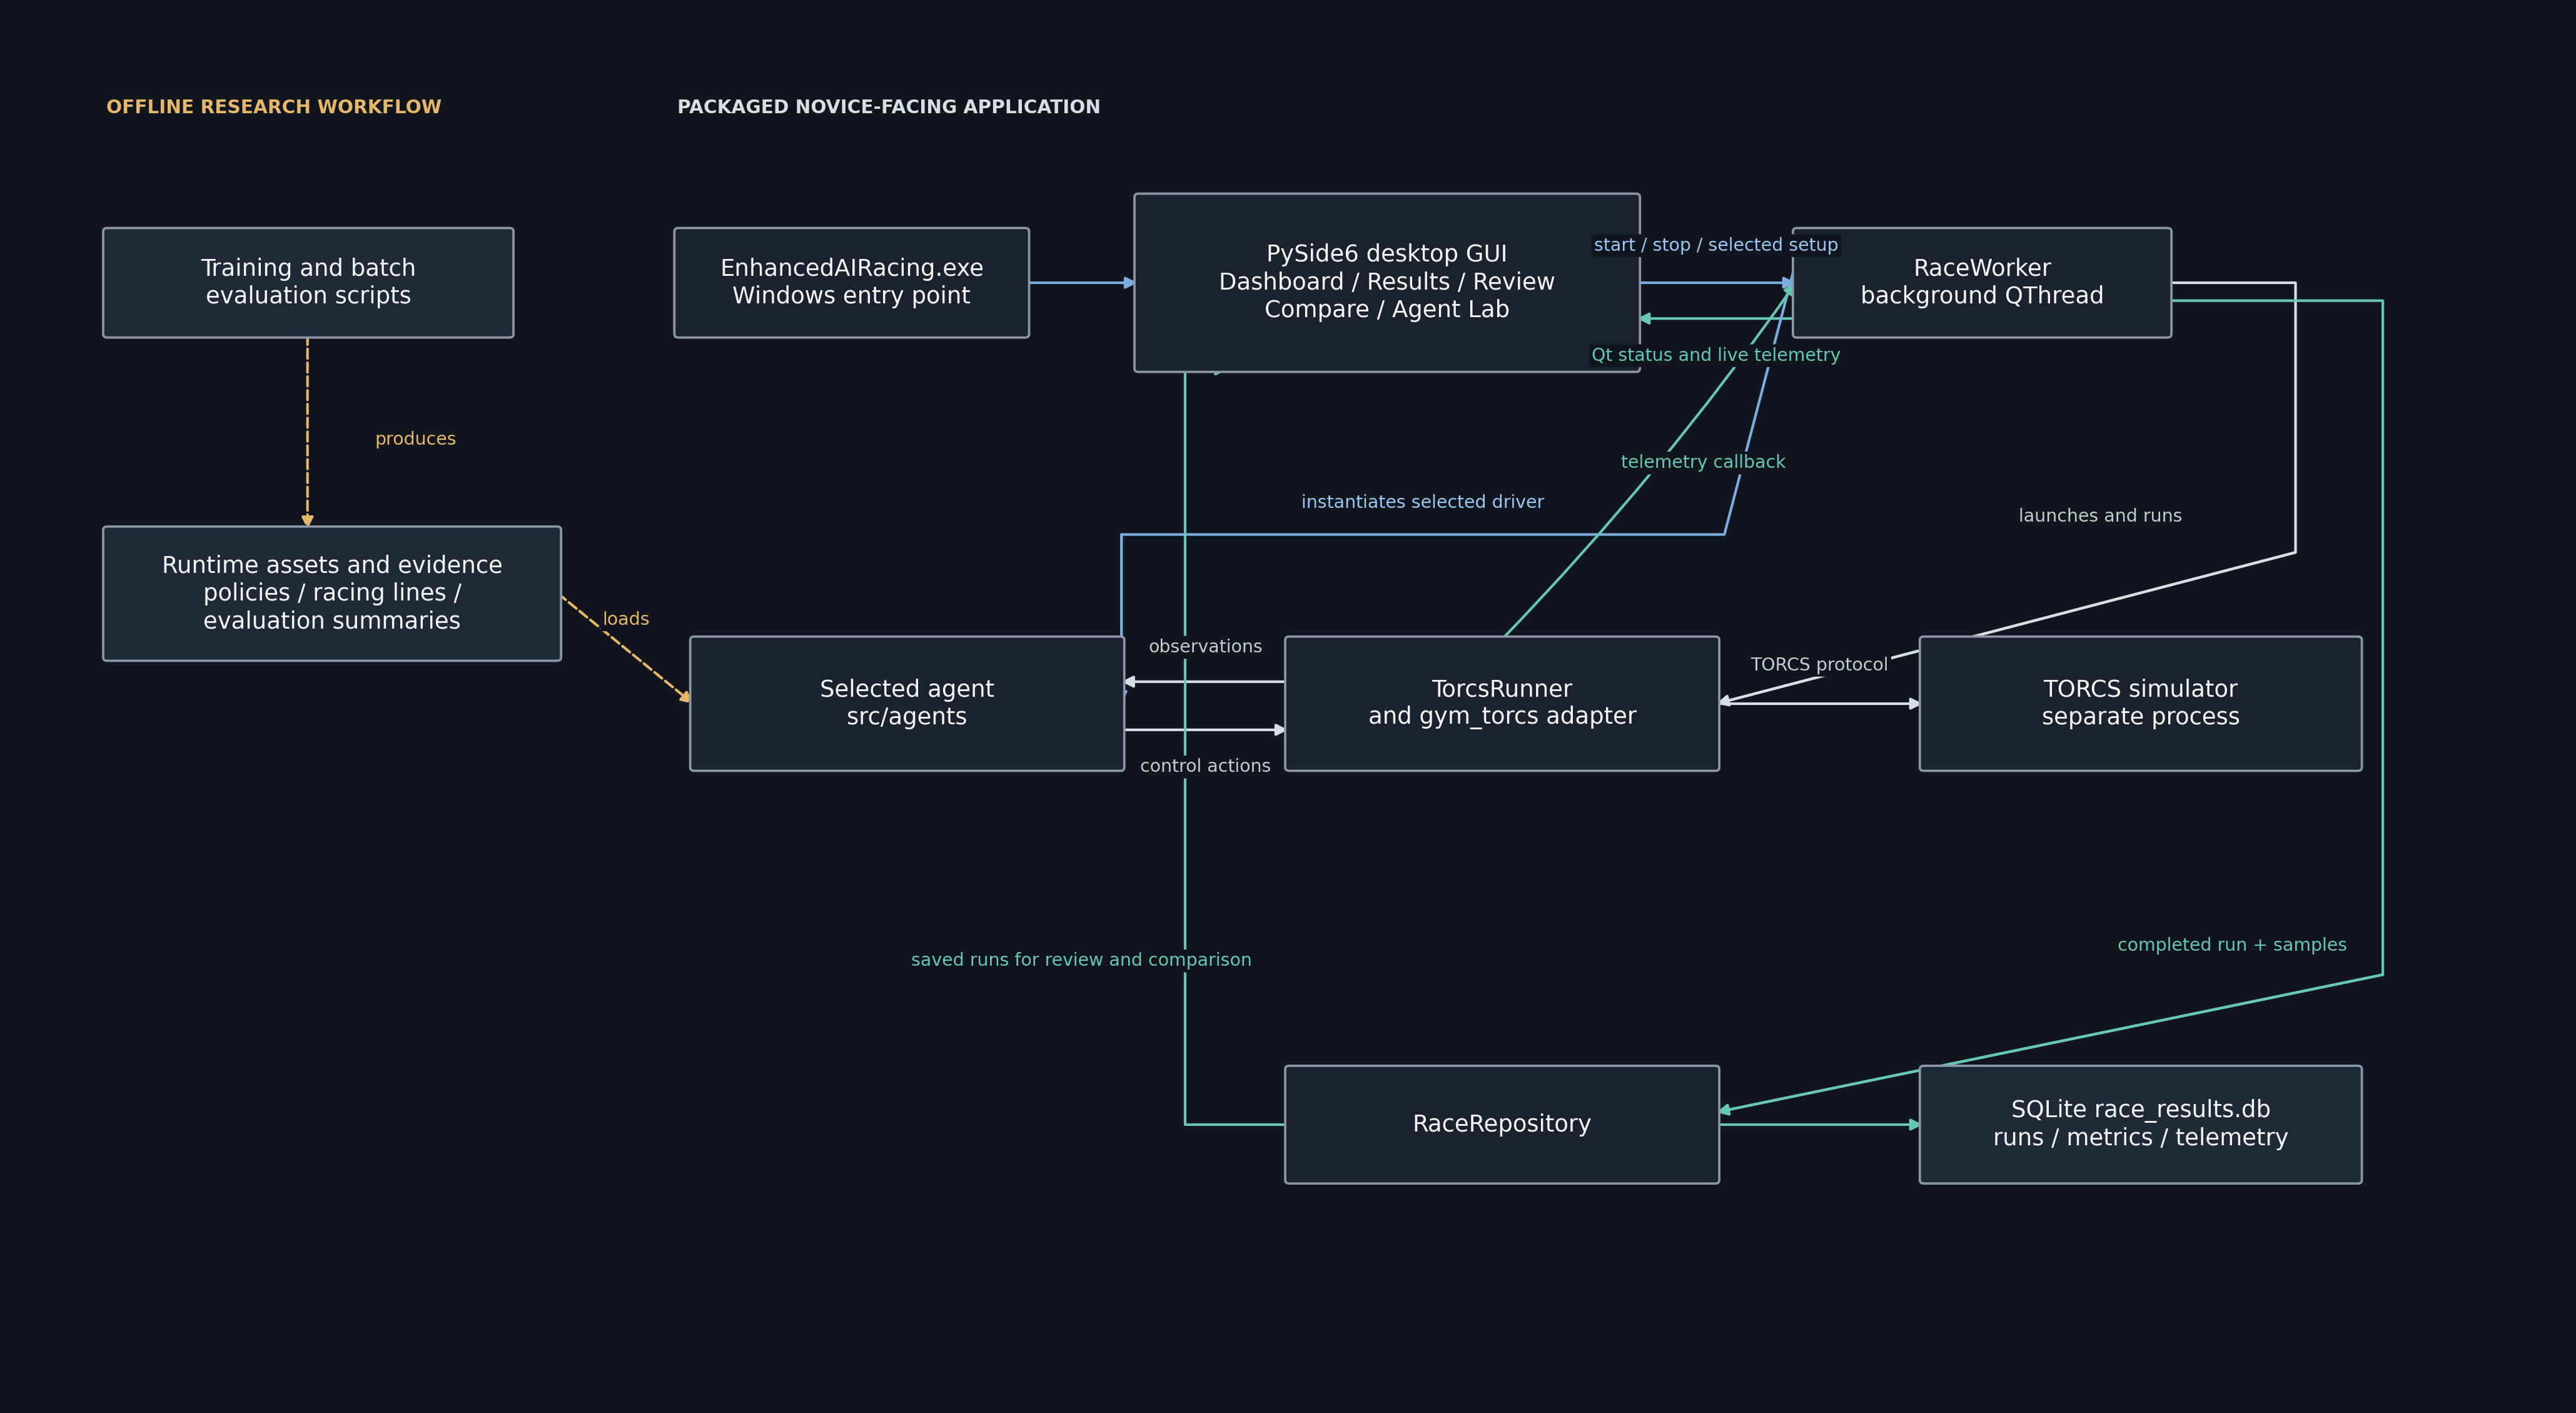
\includegraphics[width=\textwidth]{architecture-overview.png}
  \caption{System architecture of Enhanced AI Racing. The novice-facing application launches and explains fixed policies, while offline training and formal evaluation remain separate from the runtime control loop and preserve auditable evidence.}
  \label{fig:architecture-overview}
\end{figure}

This separation is not merely stylistic. Keeping the runner independent of agent logic means that a new controller can be compared without rebuilding the interface or database. Keeping the GUI independent of training means a novice can run a protected policy without accidentally modifying a checkpoint. Keeping formal evaluation scripts separate from GUI demonstrations protects evidence provenance: a visible application run is useful for explanation, whereas a fixed-policy repeated evaluation is stronger evidence of reliability.

The storage layer has two granularities. Run-level records contain agent identity, track, start time, completion status, lap timing and termination information. Telemetry records contain the values needed to reconstruct how that outcome occurred, including speed, track position and controls. The distinction supports efficient use of the interface: a comparison table can load summary records quickly, while a review screen retrieves the detailed trace only when a user asks why a run failed. It also aligns the data model with the dissertation's evidence hierarchy, where every aggregate claim should remain traceable to individual trials.

\subsection{Deployment and the novice workflow}

The release package contains the executable, its required internal runtime files, TORCS, final Agent~7 and Agent~8 policies, Dyna-Q policies, racing lines and compact results evidence. The user extracts the complete Enhanced AI Racing folder and opens \texttt{EnhancedAIRacing.exe}. The dashboard starts without a terminal; TORCS starts only after the user selects an agent and presses Start. A package smoke test verifies that the dashboard opens, expected agents appear, final policies load, TORCS launches and a completed run is visible in history.

This design directly responds to the brief's request for a launcher and beginner-facing wrapper. It also creates a clear pedagogical path: users can observe a weak random baseline, compare it with explicit rules, inspect a racing line and then encounter learned policies. The design is accessibility-oriented, including readable labels, results summaries, language support and colour choices that do not make colour the sole carrier of meaning \parencite{wcag22}. Its limitation is that the dissertation evaluates functional accessibility and explanatory design, not measured learning gains from a controlled user study.

The architecture deliberately avoids turning the novice application into a training console. Long-running learning scripts remain separate because they have different failure modes, time requirements and vocabulary from the task of observing a finished policy. The GUI exposes enough evidence to understand the result, while advanced details such as policy path and model contract are available in the research view. This division reduces cognitive load without preventing technical audit, and it avoids the misleading impression that pressing Start is equivalent to training a reinforcement-learning agent from scratch.

\section{Agent Design and Implementation}
\label{ch:agent-design}

\subsection{Shared action interface and control formulation}

All drivers are evaluated through the same closed-loop TORCS interface. At interaction $t$, a controller maps an observation $s_t$ to
\begin{equation*}
  a_t=(\delta_t,u_t,b_t,g_t),
\end{equation*}
where $\delta_t\in[-1,1]$ is steering, $u_t,b_t\in[0,1]$ are throttle and brake, and $g_t\in\{1,\ldots,6\}$ is gear. The runner applies the action, observes the next state, and records the transition $(s_t,a_t,r_t,s_{t+1})$. This common action contract prevents apparent performance differences from being caused by incompatible simulator adapters or outcome semantics.

For the learned drivers, the network action is a two-dimensional bounded vector, $z_t\in[-1,1]^2$, decoded into steering and signed longitudinal intent before throttle, brake and automatic gear selection. This retains a continuous learning action space while every agent produces lap outcomes through the same runner, database and GUI pathway.

\subsection{Baselines and engineered control}

The random agent samples bounded steering and longitudinal commands and is not expected to finish reliably. Its purpose is diagnostic: it verifies the full control path and establishes that a completed lap is not a consequence of permissive runner logic.

The rule-based anti-spin driver applies an explicit feedback law to heading $\theta_t$, normalised lateral position $p_t$, lateral speed $v_{y,t}$ and the direction $\varphi_t$ of the most open forward sensor. In its nominal mode, the implemented steering logic can be expressed as
\begin{equation*}
  \hat{\delta}_t = \frac{k_\theta\theta_t}{\pi}
  - k_p p_t + k_s\varphi_t - k_yv_{y,t},
\end{equation*}
followed by saturation, exponential smoothing and a rate limit:
\begin{equation*}
  \delta_t=\operatorname{clip}\!\left(\delta_{t-1}+
  \operatorname{clip}\!\left(\rho\delta_{t-1}+(1-\rho)\hat{\delta}_t-\delta_{t-1},
  -\Delta_t,\Delta_t\right),-\delta_{\max},\delta_{\max}\right).
\end{equation*}
The engineering problem was not merely centring the car. At speed, a reactive correction can become too large after lateral motion has accumulated, producing alternating steering, lost traction or an edge excursion. Gains and limits therefore vary with speed, edge proximity and stability state; target-speed control similarly suppresses throttle during braking or recovery. The deliberate trade-off is pace for a recoverable vehicle state.

Without the rate limit, small changes in sensor evidence can reverse a large steering command between simulator steps. Thus $\Delta_t$ imposes a discrete-time smoothness constraint: correct cross-track and heading error quickly enough to recover, but not so abruptly that the correction causes instability.

The Map-Aware Racing-Line Agent adds target track position $p_t^*$, heading offset $\theta_t^*$ and local curvature $\kappa_t$ from the stored route. Its cross-track error is
\begin{equation*}
  e_t=p_t-p_t^*, \qquad
  c_t=-\arctan\!\left(\frac{k_e e_t}{\max(v_t/3.6,4)+6}\right).
\end{equation*}
The steering command combines heading, cross-track, curvature and lateral-motion terms:
\begin{equation*}
  \hat{\delta}_t=k_\psi(\theta_t+\theta_t^*)+k_cc_t+k_\kappa\kappa_t-k_vv_{y,t}.
\end{equation*}
It is then smoothed and rate-limited using the same control constraints as the rule-based agent. The racing line addresses the reactive baseline's lack of an explicit target position through a bend. Its cost is track dependence: it is interpretable on \texttt{g-track-3}, but needs a new route representation on an unseen circuit. This implements the anticipatory planning principle noted by \textcite{quadflieg2010}.

\subsection{Dyna-Q learning agent}

Dyna-Q converts the continuous simulator state into a discrete tuple
\begin{equation*}
  \bar{s}_t=(q_t,b_v,b_p,b_\theta,b_{v_y},b_f,b_d,b_o,b_b),
\end{equation*}
where $q_t$ is lap section and the remaining bins encode vehicle and sensor conditions. The policy chooses from 26 fixed steering, throttle, brake and recovery actions. This was a pragmatic response to expensive live simulation: the tabular learner was inexpensive to inspect, save and replay. Its limitation was structural: states needing different small continuous corrections can share a bin, while a finite action table cannot express every cornering adjustment.

Action selection is $\epsilon$-greedy, with the implemented linear schedule
\begin{equation*}
  \epsilon_t=\epsilon_{\min}+(\epsilon_0-\epsilon_{\min})
  \left(1-\min\!\left(\frac{t}{T},1\right)\right),
  \quad (\epsilon_0,\epsilon_{\min},T)=(0.24,0.035,80000).
\end{equation*}
For each real transition, the temporal-difference error and update are
\begin{equation*}
  \Delta_t=r_t+\gamma(1-d_t)\max_a Q(\bar{s}_{t+1},a)-Q(\bar{s}_t,a_t),
  \qquad Q\leftarrow Q+\alpha\Delta_t.
\end{equation*}
with $\alpha=0.18$ and $\gamma=0.96$. The learned transition model additionally supplies 16 sampled planning updates per real step. The shaped reward favours progress and aligned speed while penalising unsafe states, making completion preferable to locally fast instability. Planning can reuse remembered transitions but cannot recover detail discarded by binning or create an absent action. The finalised driver sets $\epsilon=0$ and disables planning, so evaluation cannot change the table measured.

\subsection{N-step TD3: Agent 7 and Agent 8}

The TD3 observation begins with 45 normalised features: three velocities, three derived accelerations, RPM, heading, track position, 19 track-edge sensors, four wheel speeds, and racing-line difference plus look-ahead curvature slots. Three observation frames and three preceding two-dimensional actions are stacked, giving
\begin{equation*}
  \dim(s_t)=3(45)+3(2)=141.
\end{equation*}
Agent~7 populates the five route-geometry slots from the racing line. Agent~8 receives the same vehicle and sensor information but fixes those slots to zero and never loads a route file. This tests whether strong racing can be learned from local observations, although it is not a pure ablation because Agent~8 also changed reward and stability strategy.

The actor $\pi_\theta(s)$ and twin critics $Q_{\phi_1},Q_{\phi_2}$ use an N-step return. With clipped target-policy noise $\varepsilon_t$, the target is
\begin{equation*}
  \tilde{a}_{t+n}=\operatorname{clip}\!\left(\pi_{\theta^-}(s_{t+n})+\varepsilon_t,-1,1\right),
  \qquad
  y_t=\sum_{i=0}^{n-1}\gamma^ir_{t+i}+\gamma^n(1-d_{t+n})
  \min_{j\in\{1,2\}}Q_{\phi_j^-}(s_{t+n},\tilde{a}_{t+n}).
\end{equation*}
where $n=3$, $\gamma=0.992$ and $\varepsilon_t\sim\operatorname{clip}(\mathcal{N}(0,\sigma^2),-c,c)$. The critic and delayed actor objectives are
\begin{equation*}
  \mathcal{L}_Q=\mathbb{E}\!\left[(Q_{\phi_1}-y_t)^2+(Q_{\phi_2}-y_t)^2\right],
  \qquad
  \mathcal{L}_{\pi}^{\mathrm{RL}}=-\mathbb{E}\!\left[Q_{\phi_1}(s,\pi_\theta(s))\right].
\end{equation*}
Twin critics, target smoothing and policy delay reduce overestimation pressure \parencite{fujimoto2018}, but do not replace a defensible reward and evaluation protocol. Early TD3 work found locally fast behaviour without repeated completion, so selection shifted towards clean repeated laps.

N-step return is useful because corner-entry actions may have consequences several interactions later. The terminal indicator prevents value beyond failure, while the critic minimum guards against promoting actions due to one optimistic estimator.

Agent~8's stability profile adds self-imitation only from its own successful trajectories. For elite transitions $\mathcal{B}_E$, the delayed actor loss becomes
\begin{equation*}
  \mathcal{L}_{\pi}=\mathcal{L}_{\pi}^{\mathrm{RL}}+
  \lambda_k\,\mathbb{E}_{(s,a)\sim\mathcal{B}_E}\!\left[\lVert\pi_\theta(s)-a\rVert_2^2\right].
\end{equation*}
where $\lambda_k$ decays across actor updates. This is neither external demonstration nor racing-line cloning: it regularises towards rare successful actions generated by the policy itself. It addressed the failure pattern where a fast lap was surrounded by terminated trajectories, retaining clean experience while the reinforcement objective stayed active. Candidate selection prioritised completion rate, then median completed-lap time and distance. Deployment filters only steering with a reset exponential moving average, a documented runtime contract rather than hidden assistance.

Reward assigns immediate value to forward, centred and physically safe behaviour; self-imitation changes the actor only when successful actions are retained. Their separation makes the training history auditable and prevents Agent~8 being reduced to an algorithm label.

\subsection{Design comparison}

The agents encode distinct assumptions and risks. Rules trade adaptation for inspectability; racing-line control trades transfer for anticipatory reference information; Dyna-Q trades resolution for inexpensive planning; and TD3 trades training simplicity for continuous, high-dimensional capacity. These differences make the comparison explanatory rather than a list of interchangeable labels.
\section{Novice-Facing Learning Platform and Explainability}
\label{ch:telemetry-gui}

\subsection{Design objective and intended learner}

The application is a second research contribution alongside the agent comparison. It is designed as a learning platform through which an adult or university-level newcomer can launch, observe and discuss autonomous driving without prior knowledge of TORCS, Python environments, reinforcement learning or model checkpoints. This is an intended user profile, not a claim that every non-specialist will find the software equally easy to use. The design addresses two barriers that commonly prevent a novice from engaging with an AI system: deployment friction before any behaviour can be observed, and opaque output once it is running.

The aim is therefore not to replace a formal machine-learning course or to promise that a user will understand every neural-network parameter. It is to support initial AI-literacy questions in an observable setting: What information does an agent receive? What action did it take? What happened next? Why can a fast attempt still be a poor result? Long and Magerko's framework treats understanding AI capabilities, limitations and operation as core parts of AI literacy \parencite{long2020}. Enhanced AI Racing translates these questions into the concrete consequences of steering, throttle, braking, track position and lap completion.

The design also follows human-AI interaction guidance that users should be able to understand system status, capability and limitation \parencite{amershi2019}. In this context, that means a learner should not see Agent~8 presented as an unexplained high score. The interface instead makes visible the distinction between an explicit rule, a route-informed controller and a learned policy; between a completed lap and a failure; and between an exceptional fastest lap and behaviour that repeats across attempts. These are pedagogical design choices, not claims of direct access to every internal neural-network decision.

\subsection{Staged learner workflow}

The platform uses a staged workflow so that a learner can begin with familiar actions before encountering specialist terminology. The first screen presents agent, track and car selection beside a Start control. The release package supplies TORCS, runtime files and fixed policies, so this first step does not require installation of Python packages, manual configuration of a simulator path or discovery of a checkpoint. Figure~\ref{fig:live-dashboard} shows the Live Telemetry dashboard before a race begins. The Dyna-Q selection is deliberate: the visible Observe, Act, Reward, Update and Replay stages provide an approachable bridge from what the car is doing to the idea of reinforcement learning.

\begin{figure}[htbp]
  \centering
  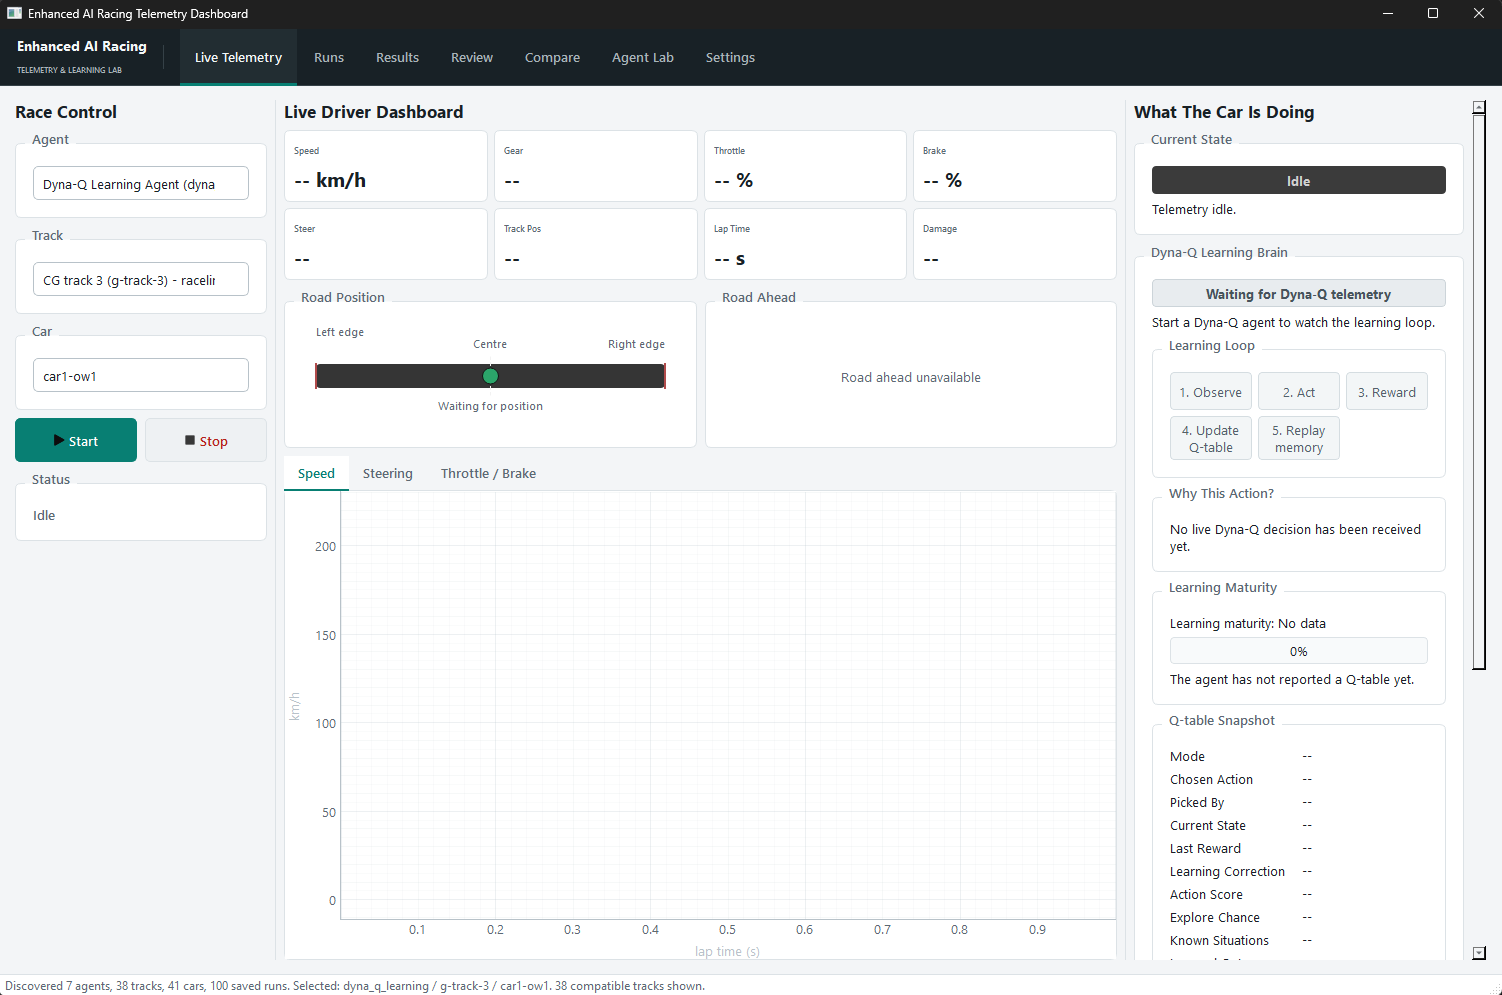
\includegraphics[width=\textwidth]{figure_8_1_live_dashboard.png}
  \caption{Live Telemetry dashboard with agent, track and car selection, live controls, readable road-position indicators and the Dyna-Q learning-loop explanation. Source: Enhanced AI Racing application.}
  \label{fig:live-dashboard}
\end{figure}

The intended learning sequence is summarised in \cref{tab:novice-workflow}. It is not a linear tutorial that forces a user through every screen. Rather, it gives a useful first route through the system and a structure for an instructor-led demonstration. The random, rule-based and map-aware agents are important at the start of this route: they make the observable relationship between information, control and outcome clearer before a learner encounters the more complex TD3 policies.

\begin{table}[htbp]
  \centering
  \caption{Research-informed workflow through the novice-facing learning platform.}
  \label{tab:novice-workflow}
  \small
  \begin{tabularx}{\textwidth}{p{0.18\textwidth}p{0.25\textwidth}YY}
    \toprule
    Stage & Learner question & Interface evidence & Intended AI-literacy outcome \\
    \midrule
    Launch and select & Can I run an AI driver without development setup? & Packaged executable, agent selector and Start control & Distinguish running a fixed policy from writing or training one \\
    Observe & What is the car sensing and doing now? & Live speed, controls, road position, road-ahead indicators and state labels & Relate observations to sequential driving actions \\
    Review & Why did this individual run succeed or fail? & Saved-run summary, termination information, replay timeline and telemetry traces & Treat behaviour as evidence rather than as a single score \\
    Compare & Is the fastest displayed lap also the most reliable result? & Trial count, completion rate, median completed-lap time and visible failures & Interpret capability, repeatability and uncertainty together \\
    Explain & How do the agents differ? & Agent Lab descriptions of signals, decision process, strengths and failure signs & Compare rules, route information and learned policies without assuming equivalence \\
    \bottomrule
  \end{tabularx}
\end{table}

\subsection{Telemetry, progressive disclosure and evidence literacy}

Telemetry is the bridge between technical evaluation and novice explanation. Each stored run preserves speed, position, heading, steering, throttle, braking, progress, lap timing and termination information. Those values answer different questions at different levels of detail. A learner can begin with an outcome label such as \enquote{completed} or \enquote{off track}, while a more advanced user can inspect the corresponding steering or throttle trace. This progressive disclosure reduces initial cognitive load without removing the evidence needed for technical audit.

Figure~\ref{fig:run-review} illustrates this relationship in the Review workspace. A completed Agent~8 run is shown with a summary, a time-based replay, direct state values, road-position and road-ahead indicators, telemetry charts, and plain-language \enquote{What the Car Is Doing} and \enquote{Why} panels. The explanation does not assert a complete causal account of the neural policy. It connects observable state and action to the current driving situation, which is a more honest and useful form of explanation for a sequential deep-learning system.

\begin{figure}[htbp]
  \centering
  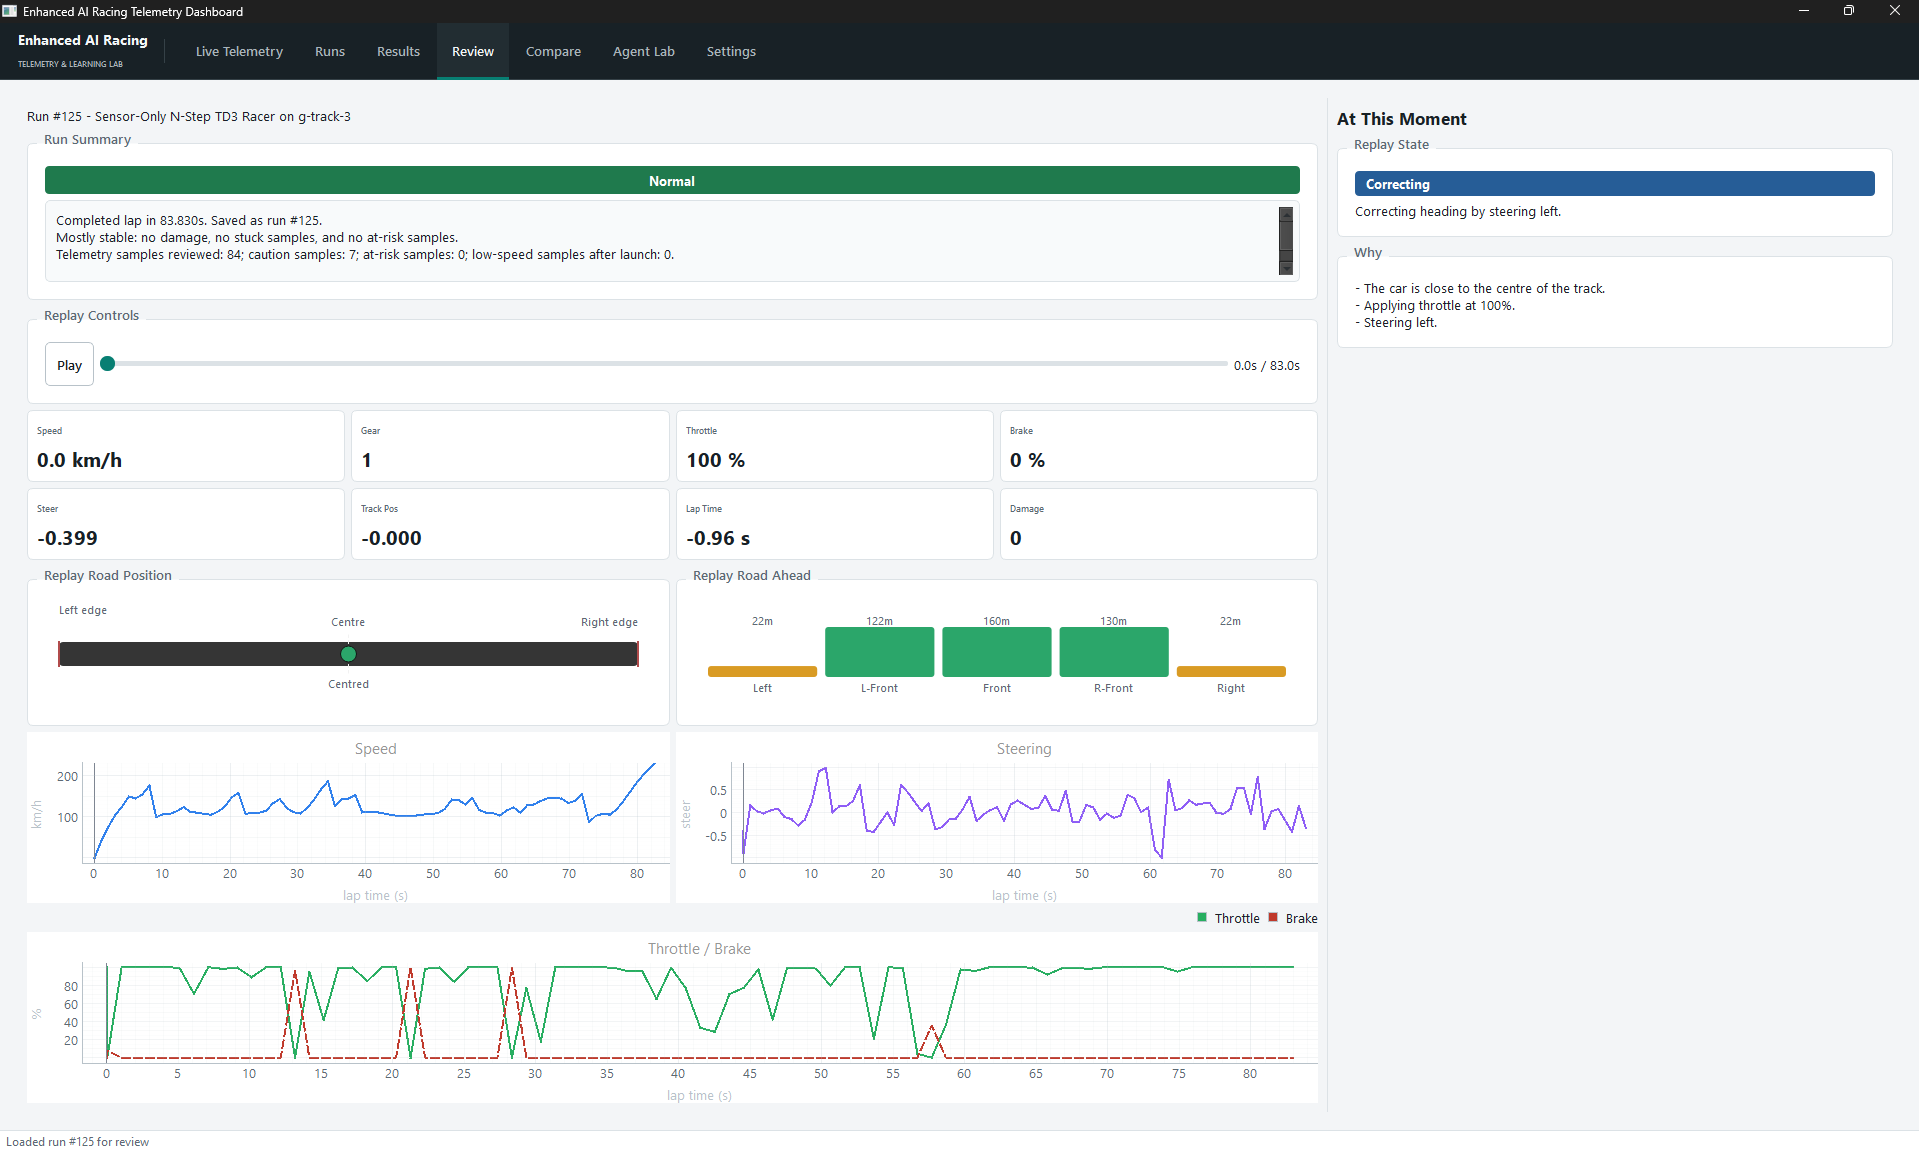
\includegraphics[width=\textwidth]{figure_8_2_run_review.png}
  \caption{Review workspace for a saved Agent~8 run. Summary, replay controls, current telemetry and plain-language state explanations allow a learner to connect an outcome to the underlying trace. Source: Enhanced AI Racing application.}
  \label{fig:run-review}
\end{figure}

The Results and Compare workspaces apply the same principle to aggregate evidence. Completion is shown with its denominator; median completed-lap time describes typical pace only among finished attempts; fastest time is presented as capability, not reliability; and failures remain visible. These reporting choices implement the reliability concerns discussed by \textcite{henderson2018} and \textcite{agarwal2021} in a form that a novice can inspect. The detailed research view retains policy and evaluation provenance, so simplified presentation does not collapse different batches into a misleading single ranking.

Agent Lab provides the conceptual bridge between these screens. It explains what each agent observes, how it selects actions, its strengths and common failure signals. The presentation order is intentional: a user can observe random behaviour, then explicit rules, then route-aware control, before considering policies that learn from reward. This grounds abstract terms such as exploration, reward and policy in visible differences in driving behaviour. Language support, readable labels and visual signals that do not rely on colour alone further support access, in line with the accessibility considerations of \textcite{wcag22}.

\subsection{Functional evidence and boundary of the claim}

The novice-facing claim is evaluated through functional evidence rather than a participant study. The release smoke test checks the concrete workflow represented in \cref{tab:novice-workflow}: the dashboard opens from the packaged folder; expected agents and policies are available; TORCS starts from the interface; a user can initiate a run; and a completed outcome is retained for later review. Together with automated checks of the GUI models, results storage and explanation content, this demonstrates that the designed learning route exists in the delivered software rather than only in a prototype mock-up.

This is meaningful but bounded evidence. It supports the claim that the platform reduces setup barriers and is designed to help a novice inspect how agents drive, fail and differ. It does not establish effectiveness, efficiency or satisfaction for a defined population of adults or students, nor does it measure whether a learner can accurately explain reinforcement learning after use. Those stronger claims require a small task-based study with intended users, for example asking participants to launch an agent, identify why a run failed and interpret a completion-rate comparison. The current contribution is consequently a research-informed, evidence-aware learning platform with functional accessibility, not a validated educational intervention.
\section{Testing and Experimental Setup}
\label{ch:testing}

\subsection{Verification strategy}

Verification was layered because a defect in one component can corrupt later experimental evidence. Unit tests cover behaviour that does not require a live simulator, including Dyna-Q state encoding and value updates, map-aware steering calculations, lap timing, telemetry conversion, repository persistence and GUI explanation models. Integration tests then exercise the full agent-environment loop: TORCS supplies observations, the selected driver returns actions, the runner maintains the race session and the storage layer records the resulting evidence. The GUI path is tested by starting a race, receiving live updates and confirming that a stored outcome can be reviewed afterwards.

This division matters methodologically. A successful live lap is not proof that the result repository recorded the correct time, and a correct database record is not proof that the agent received valid observations. Lap timing, completion checks and repository retrieval were therefore verified separately from live TORCS integration. The result is a more credible chain from simulator state to the numbers reported in \cref{ch:results}.

The Windows build adds a deployment-focused smoke test. It checks the packaged TORCS path, project discovery, racing-line assets and the final Agent~7 and Agent~8 policies before a release folder is produced. The release check then confirms that the dashboard opens without a development console, expected agents are visible, a selected policy loads, TORCS starts from the interface and a completed run appears in the results workspace. This verifies the novice-facing runtime rather than only the author's development configuration.

\subsection{Functional evaluation of the novice workflow}

The learning-platform claim was evaluated as a set of observable workflow conditions, rather than by assuming that the presence of a GUI proves usability. \Cref{tab:novice-acceptance} identifies the required tasks and their functional evidence. These conditions test whether the delivered application provides a coherent route from launching a selected agent to interpreting its recorded outcome. They do not test whether an intended user completes the route efficiently, enjoys it or learns a specified concept; those questions require participant-based methods.

\begin{table}[htbp]
  \centering
  \caption{Functional acceptance evidence for the novice-facing workflow.}
  \label{tab:novice-acceptance}
  \small
  \begin{tabularx}{\textwidth}{p{0.11\textwidth}p{0.30\textwidth}YY}
    \toprule
    ID & Acceptance task & Expected outcome & Evidence in the delivered system \\
    \midrule
    NF1 & Open the packaged application. & Dashboard opens without a terminal or Python environment. & Release smoke test and the dashboard shown in \cref{fig:live-dashboard}. \\
    NF2 & Select a named agent and start a race. & TORCS launches through the GUI with the selected controller. & Agent, track and car controls; runtime and runner integration checks. \\
    NF3 & Review a saved outcome. & Summary, termination information and telemetry are retrievable after a run. & SQLite-backed run history and the Review workspace in \cref{fig:run-review}. \\
    NF4 & Compare outcomes. & Pace, completion count, failure and provenance remain visible together. & Results and Compare workspaces; stored application and repeated-evaluation records. \\
    NF5 & Read an agent explanation. & Plain-language guide identifies information source, decision approach and failure signals. & Agent Lab explanation models and automated content checks. \\
    \bottomrule
  \end{tabularx}
\end{table}

\subsection{Controlled race scenario}

The core evaluation scenario was fixed: the \texttt{g-track-3} circuit, the same car and one circuit per attempt. The same runner semantics were used across agents. A completed lap required the timing system to record a full circuit within the configured episode limit. The runner also recorded off-track behaviour, reverse driving, stalling, damage and termination reason. These events were retained as evidence of stability or failure; a terminated or timed-out attempt was not recoded as a completed lap.

This common scenario makes agent outcomes comparable at the level intended by the project. It removes simple environmental explanations for a difference in lap time, such as changing vehicle or circuit. It does not remove every difference between agents: the agents use different information, control methods and, for learning agents, different training histories. That distinction is deliberate. The experiment compares implemented controllers, not an abstract algorithm with every other variable held constant.

For a frozen-policy evaluation, the checkpoint was selected before the repeated batch began. Exploration and learning were disabled, and TORCS was restarted between attempts. This prevents evaluation from benefiting from online learning, persistent simulator state or an undisclosed later checkpoint. Stored GUI database runs followed the same track, car, one-lap and outcome semantics, but interactive application records and formal repeated batches remain separately labelled because their sample sizes and provenance differ.

\subsection{Measures and interpretation rules}

The principal reliability measure was completion rate:
\begin{equation*}
  CR = \frac{N_{\text{completed}}}{N_{\text{attempted}}}.
\end{equation*}
Failures remain in the denominator. This is important because a policy that records one fast successful lap but fails most attempts is not an effective racing controller. Completed-lap time was reported only for attempts that actually completed. The median completed-lap time describes typical pace conditional on success; it is not an all-run average and does not hide failure behind an arbitrarily large time. Best lap is retained as a capability indicator, while off-track, reverse, stall and termination data provide additional evidence about how a policy reached or failed to reach the finish.

The evaluation follows the reporting concerns raised by \textcite{henderson2018} and \textcite{agarwal2021}. Every result table reports attempt count with the completion proportion, and the application distinguishes a visually demonstrated run from a repeated fixed-policy evaluation. Formal confidence intervals are not manufactured from small heterogeneous batches. Instead, the dissertation reports the raw denominator, completion count, median and provenance needed for a reader to judge the evidence.

\begin{table}[htbp]
  \centering
  \caption{Evaluation measures and their role in interpretation.}
  \label{tab:evaluation-measures}
  \small
  \begin{tabularx}{\textwidth}{p{0.27\textwidth}YY}
    \toprule
    Measure & Interpretation & Reason for inclusion \\
    \midrule
    Completed laps / attempts & Reliability across the observed batch & Prevents failures being omitted \\
    Median completed-lap time & Typical pace when the policy succeeds & Less sensitive than a mean to a slow recovery lap \\
    Fastest completed lap & Demonstrated capability & Not used alone to claim reliability \\
    Off-track, reverse, stall and termination events & Failure mechanism and stability context & Explains why a lap was not completed \\
    Telemetry trace & Time-series evidence of state and action & Supports diagnosis and novice explanation \\
    \bottomrule
  \end{tabularx}
\end{table}

\subsection{Validity and residual limits}

The strongest remaining internal threat is training and selection sensitivity. Reward definitions, observation contracts, training distributions, candidate selection and tuning effort all influence a learned policy. The project reduces ambiguity by preserving policy paths and documenting Agent~7 and Agent~8 contracts, but this does not turn their comparison into a pure ablation of racing-line input. The next controlled study would hold reward, training budget and selection procedure fixed while changing only the geometry features.

The principal external threat is track dependence. A map-aware controller may need a new racing line on a new circuit, while the sensor-only policy has not demonstrated transfer beyond \texttt{g-track-3}. The study also has unequal sample sizes: two application runs support a weaker reliability claim than forty repeated evaluations, even if both occur under the common scenario. These limits are disclosed rather than treated as reasons to discard the results. Finally, the interface is functionally tested but not assessed through a novice participant study. The project therefore demonstrates accessible deployment and inspectable evidence, not verified learning outcomes.

\section{Results}
\label{ch:results}

\subsection{Evidence overview}

The results examine whether the agents complete the common racing task and whether the application preserves interpretable evidence. \Cref{tab:agent-results} separates application database records from repeated frozen-policy evaluations: the former demonstrate integrated behaviour, while the latter provide stronger reliability evidence. All use the common \texttt{g-track-3}, car and one-lap scenario described in \cref{ch:testing}.

\begin{table}[htbp]
  \centering
  \caption{Agent performance under the common one-lap \texttt{g-track-3} scenario. Database records and repeated fixed-policy evaluations are intentionally reported as separate evidence sources.}
  \label{tab:agent-results}
  \small
  \begin{tabularx}{\textwidth}{p{0.22\textwidth}p{0.18\textwidth}p{0.07\textwidth}p{0.08\textwidth}p{0.11\textwidth}YY}
    \toprule
    Agent & Evidence source & Attempts & Completed & Completion rate & Best completed lap & Median completed lap \\
    \midrule
    Rule-Based Anti-Spin & Application database & 2 & 2 & 100\% & 98.394 s & 99.142 s \\
    Map-Aware Racing-Line & Application database & 15 & 15 & 100\% & 90.958 s & 92.056 s \\
    Dyna-Q Learning & Application database & 3 & 1 & 33.3\% & 305.562 s & 305.562 s \\
    TD3 Scratch & Application database & 6 & 0 & 0\% & N/A & N/A \\
    Agent 7 N-step TD3 v3 & Repeated evaluation & 20 & 18 & 90\% & 103.230 s & 104.220 s \\
    Agent 7 N-step TD3 v4 & Repeated evaluation & 10 & 10 & 100\% & 103.386 s & 103.887 s \\
    Agent 8 Sensor-Only TD3 & Repeated evaluation & 40 & 36 & 90\% & 83.038 s & 83.038 s \\
    \bottomrule
  \end{tabularx}
\end{table}

\subsection{Engineered baselines and early learning results}

\Cref{fig:completion-reliability} reports completion proportion, its 95\% Wilson interval and the raw denominator, so 2/2 is not treated as equally certain as 36/40. The Map-Aware Racing-Line Agent completed all 15 stored attempts, with no off-track events and a 92.056-second median lap. It is therefore a substantive benchmark: explicit route knowledge and engineered control were both fast and reliable on the known circuit. The rule-based agent also completed 2/2, but that small batch supports only a weak reliability claim.

\begin{figure}[htbp]
  \centering
  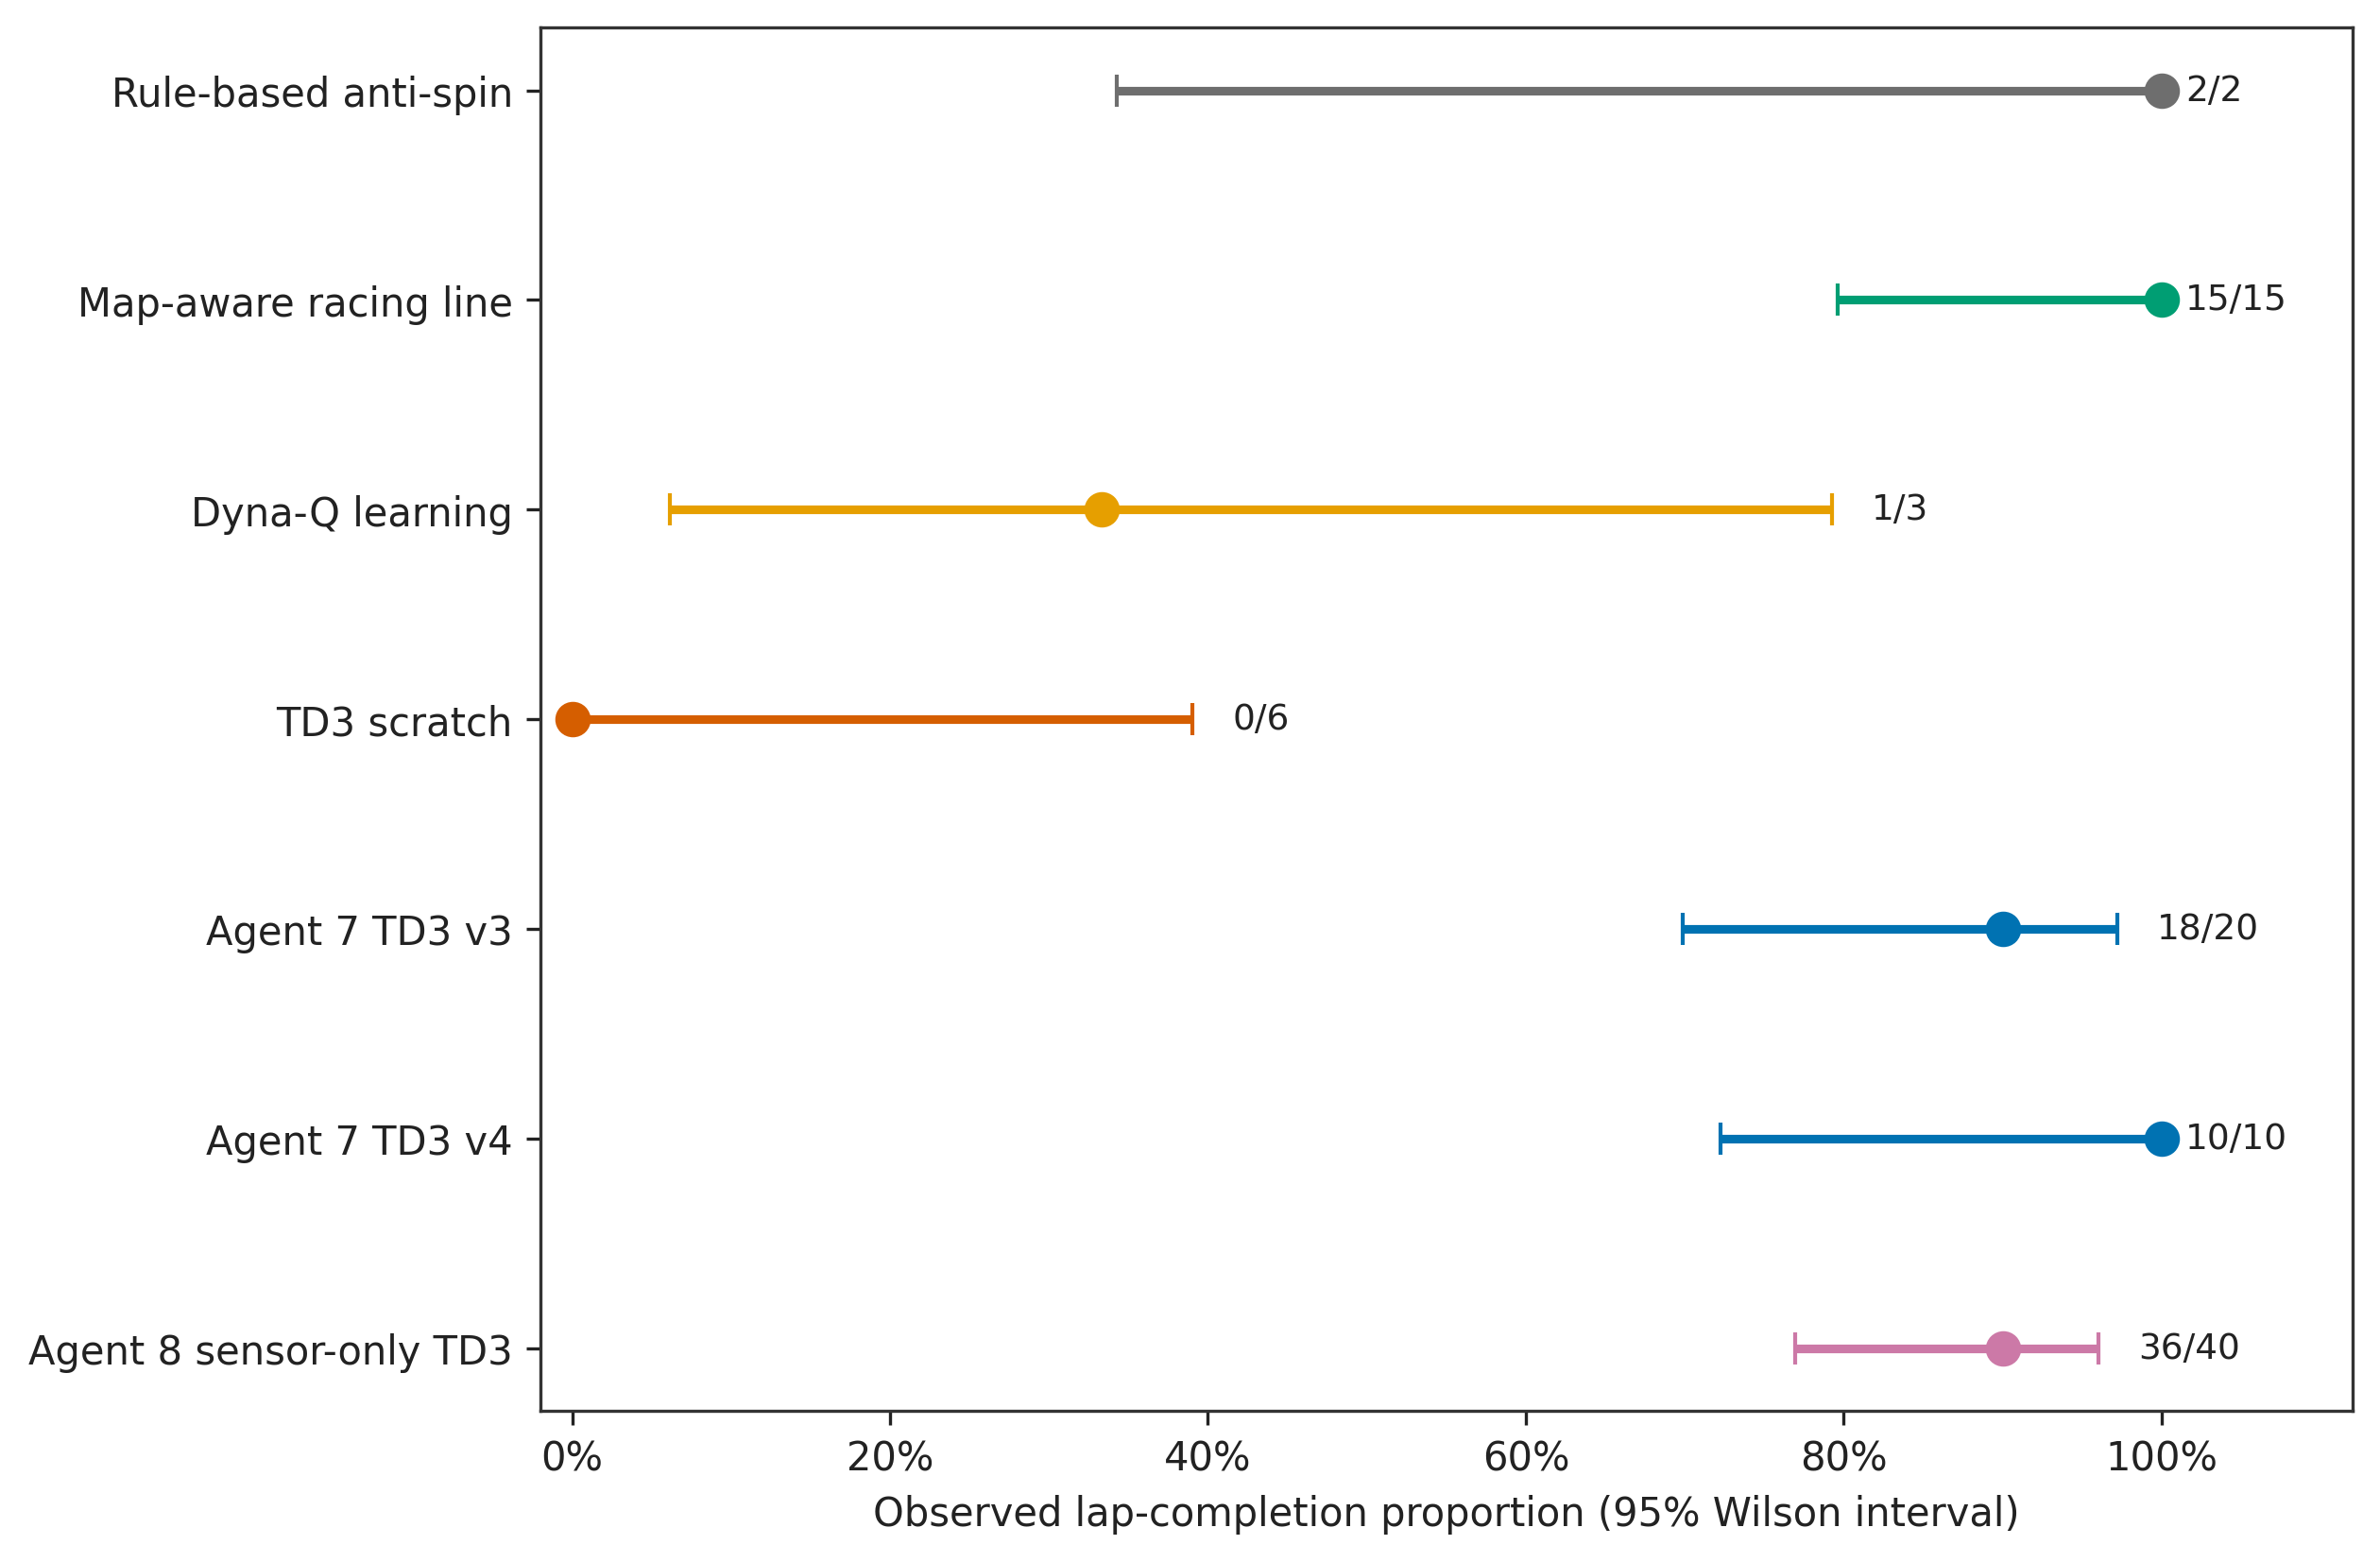
\includegraphics[width=0.90\textwidth]{figure_10_1_completion_reliability.png}
  \caption{Observed lap-completion proportions with 95\% Wilson intervals. Labels retain completed and attempted laps, so small perfect batches are not interpreted as equally certain as larger repeated evaluations. Source: project evaluation records.}
  \label{fig:completion-reliability}
\end{figure}

The early learning results reject the assumption that a more complex algorithm automatically wins. Dyna-Q completed 1/3 at 305.562 seconds, while scratch TD3 completed 0/6. These results expose the limits of coarse discretisation and immature continuous control, and motivate repeated completion rather than a single fast event as the final selection criterion.

\subsection{Learned-policy performance}

\Cref{fig:lap-time-distribution} retains every completed-lap observation rather than reducing each group to its fastest result; failed attempts remain in \cref{fig:completion-reliability}. Agent~7 established repeated learned completion: v3 completed 18/20 at a 104.220-second median, and v4 completed 10/10 at 103.887 seconds. Both batches were slower than the map-aware benchmark.

\begin{figure}[htbp]
  \centering
  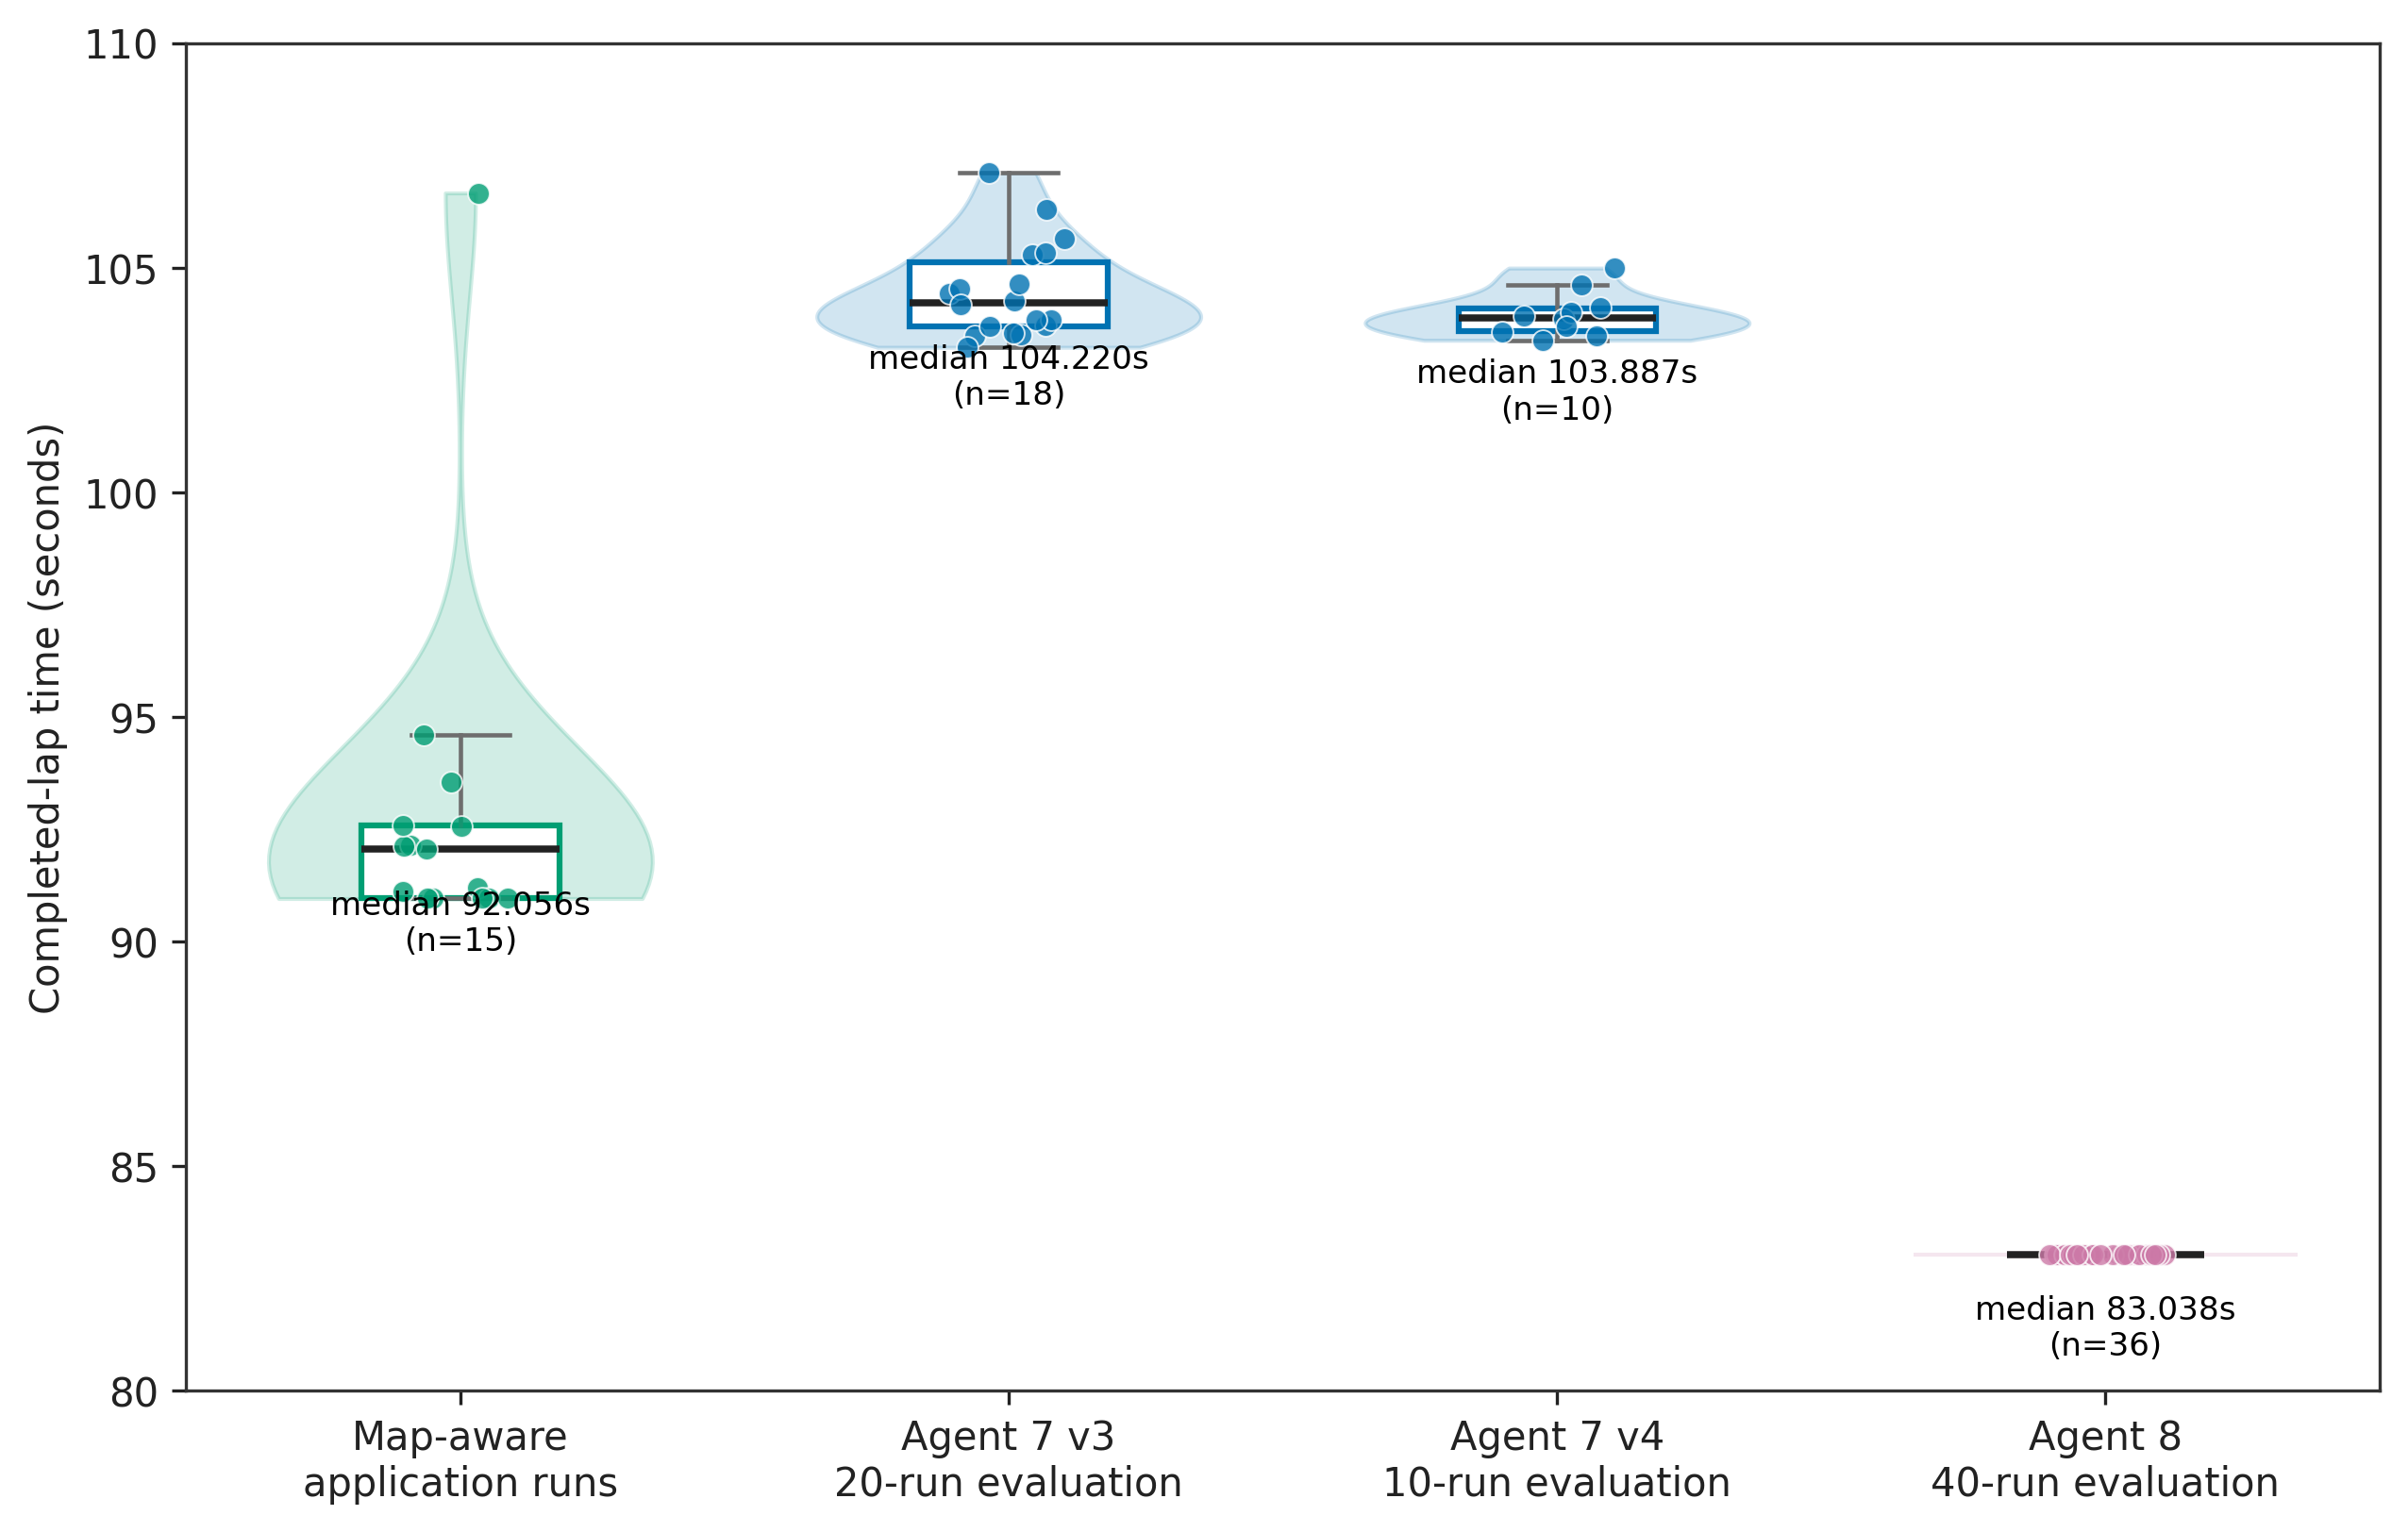
\includegraphics[width=0.90\textwidth]{figure_10_2_lap_time_distribution.png}
  \caption{Completed-lap time distributions. Individual points are retained alongside the median and interquartile range; the plot excludes failures because those attempts have no completed-lap time. Dyna-Q is reported in \cref{tab:agent-results} but omitted here because it has only one completed lap. Source: project evaluation records.}
  \label{fig:lap-time-distribution}
\end{figure}

\begin{figure}[htbp]
  \centering
  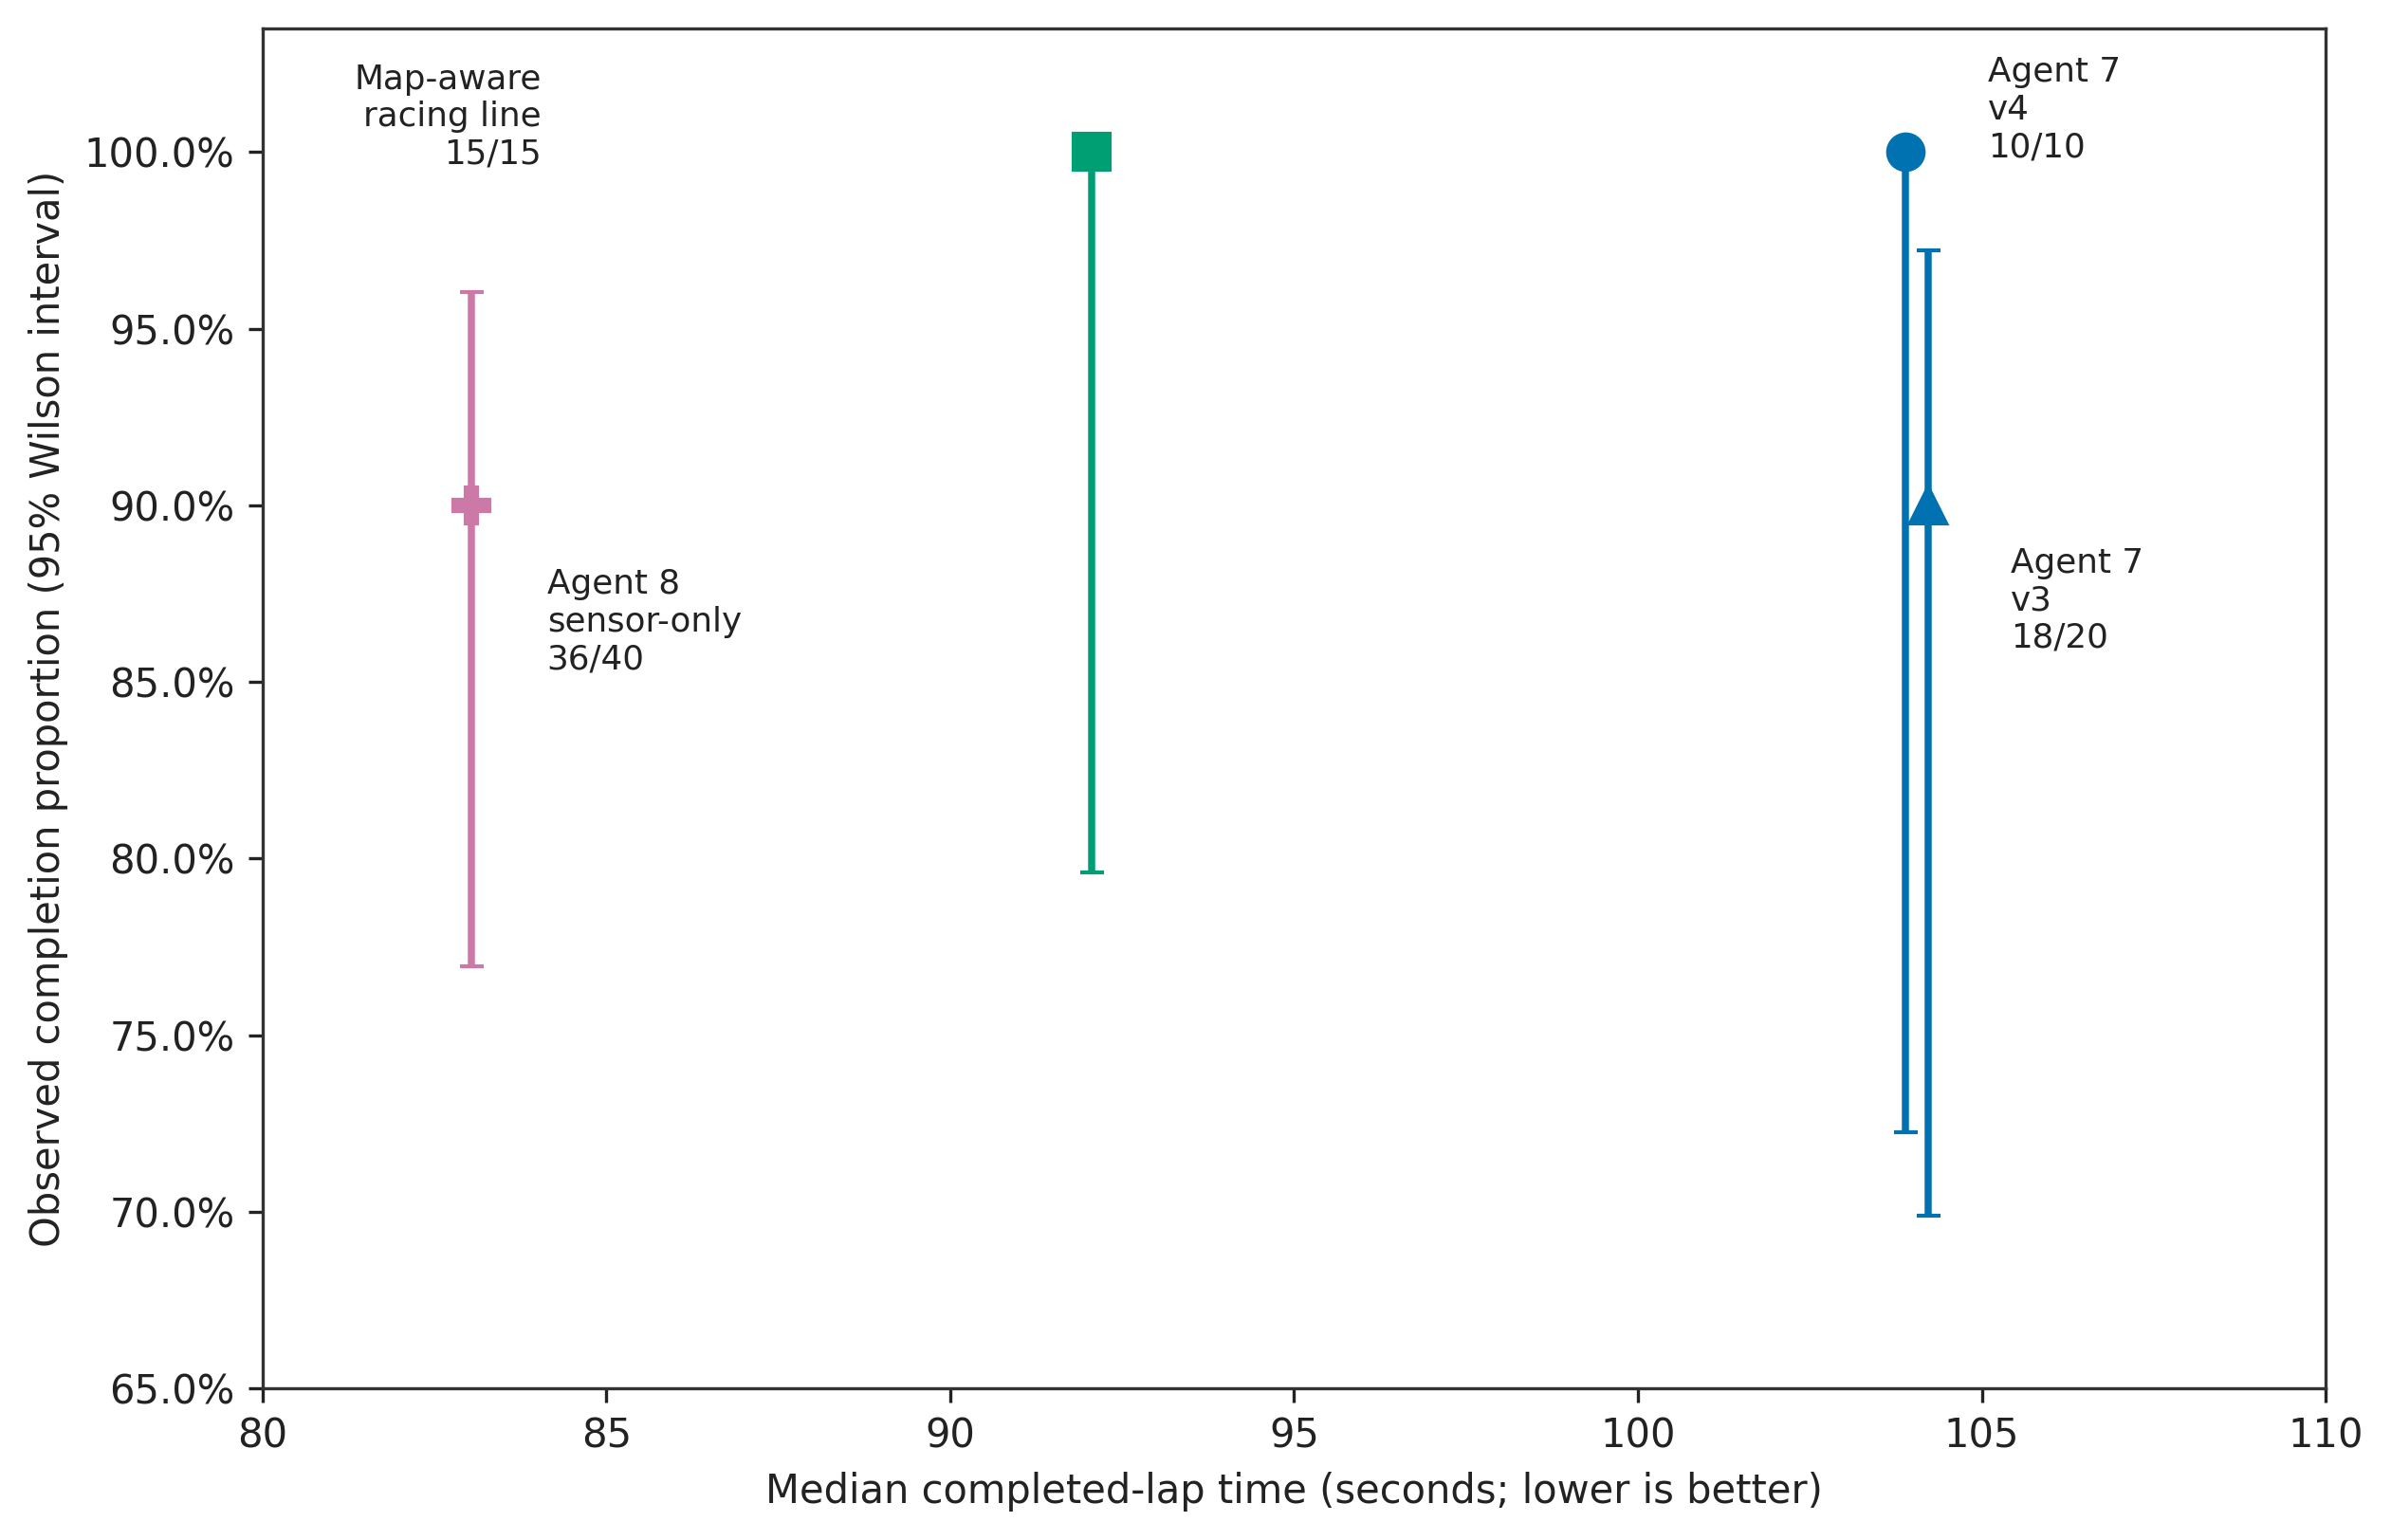
\includegraphics[width=0.90\textwidth]{figure_10_3_performance_map.png}
  \caption{Pace-reliability map for primary repeated batches with at least ten attempts. Vertical intervals are 95\% Wilson intervals for completion; horizontal positions are medians of completed laps. The map is a compact decision view rather than a claim of a controlled ablation between Agent~7 and Agent~8. Source: project evaluation records.}
  \label{fig:performance-map}
\end{figure}

Agent~8 produced the strongest observed learned result: 17/20 and 19/20 completions across two repeated batches, or 36/40 overall. Its best and median completed-lap time were both 83.038 seconds, indicating tightly clustered successful records but not erasing its four failures.

Agent~7 uses racing-line context, whereas Agent~8 uses sensors and history without an explicit route. Agent~8 therefore shows that a sensor-only policy can find an effective local strategy on \texttt{g-track-3}; it does not prove that racing-line information is unhelpful, because reward and training history also differ.

\subsection{Agent 8 version history}

\Cref{fig:agent8-development} retains the material design milestones behind the final result. It is a categorical evidence ladder, not a continuous training curve, because each point is a frozen policy after a different design decision. The v1 base completed 0/10; first completion reached 5/20 at 141.264 seconds; a pace candidate reached 2/20 at 87.299 seconds; and a stability candidate reached 5/20 at 83.118 seconds. Robust-pace and steering-limit trials both returned 0/20. The early self-imitation candidate completed 1/20 before the final champion reached 36/40 at 83.038 seconds.

\begin{figure}[htbp]
  \centering
  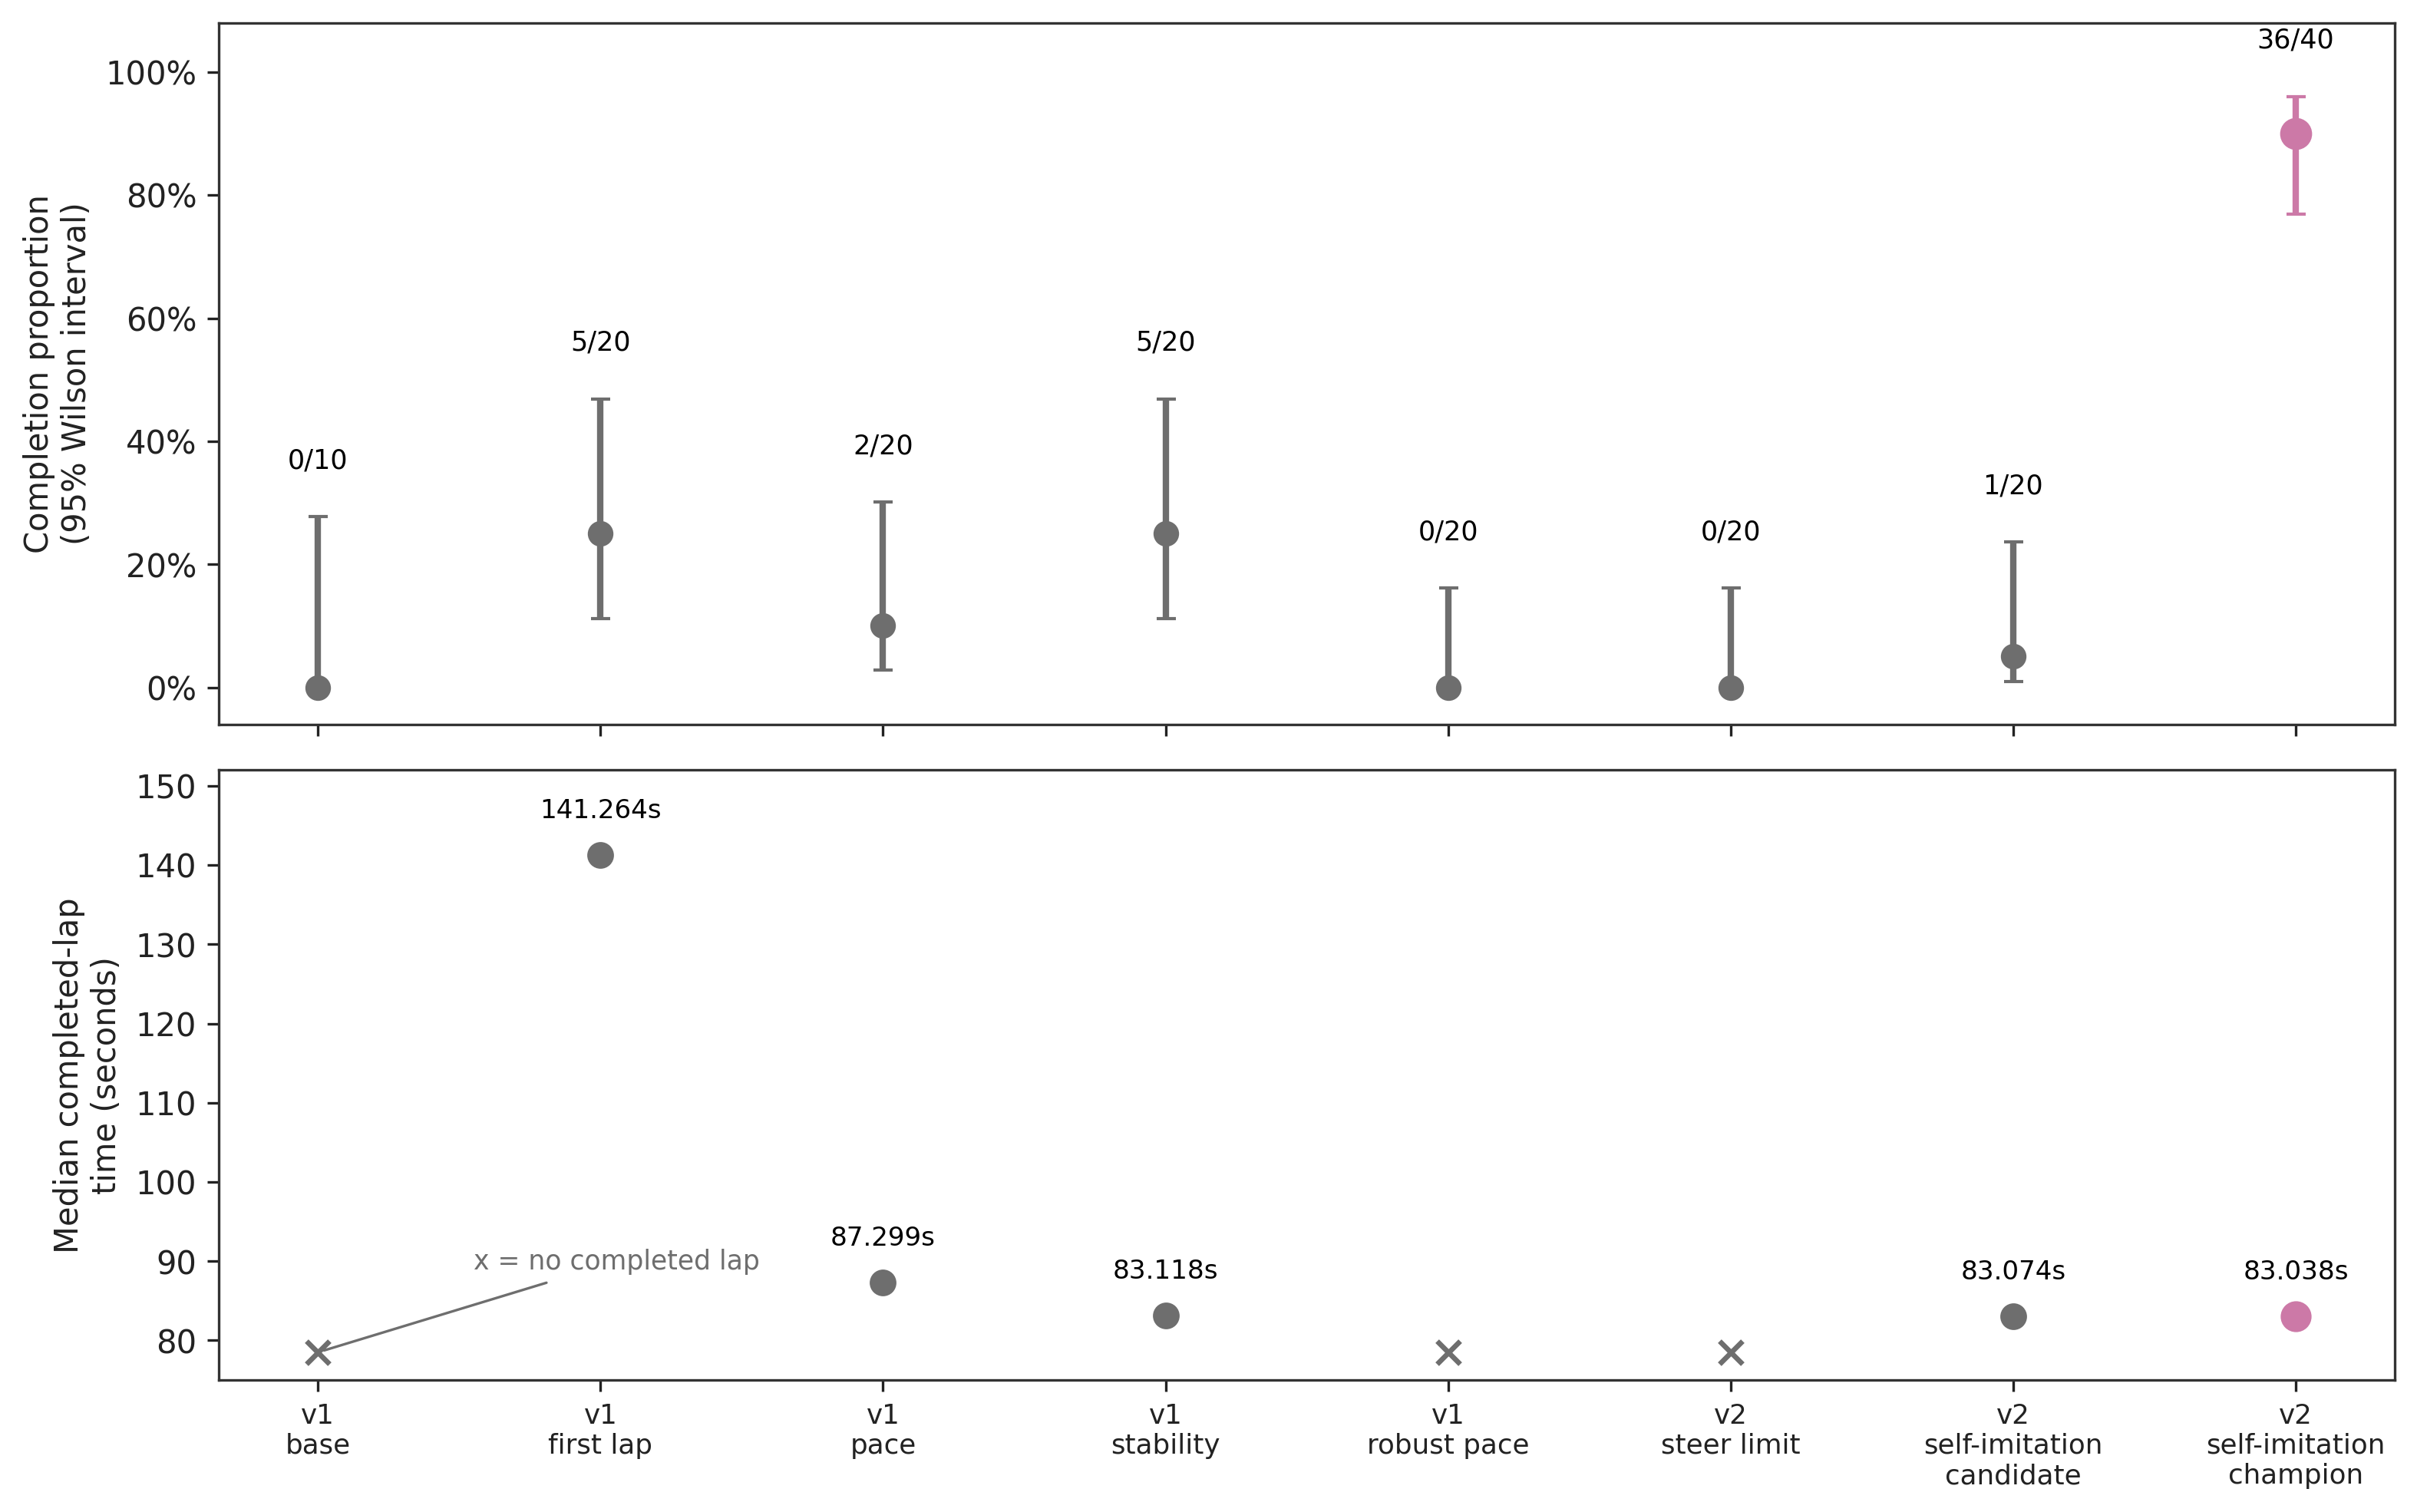
\includegraphics[width=\textwidth]{figure_10_4_agent8_development.png}
  \caption{Agent~8 material design milestones. Each categorical point is a separately evaluated frozen checkpoint or candidate; vertical intervals are 95\% Wilson intervals for completion. Crosses mark evaluations with no completed lap. The figure records changing designs and evidence, rather than implying a continuous common-budget learning curve. Source: project evaluation records.}
  \label{fig:agent8-development}
\end{figure}

The history shows that pace appeared before reliability and that apparently sensible interventions could fail under repeated evaluation. The final self-imitation and stability-oriented configuration was retained because it combined the fastest observed laps with materially stronger completion evidence. This remains a project-specific result on one track.

\subsection{Representative control behaviour}

Aggregate outcomes cannot explain how the controllers drove. \Cref{fig:control-profiles} therefore plots speed, lateral position and actions against normalised progress for three representative completed laps: the map-aware median (92.056 seconds), an Agent~7 v3 lap close to its 104.220-second median (104.180 seconds), and an 83.038-second Agent~8 lap. The traces are descriptive, resampled to common progress and lightly smoothed for legibility; raw telemetry remains stored.

\begin{figure}[htbp]
  \centering
  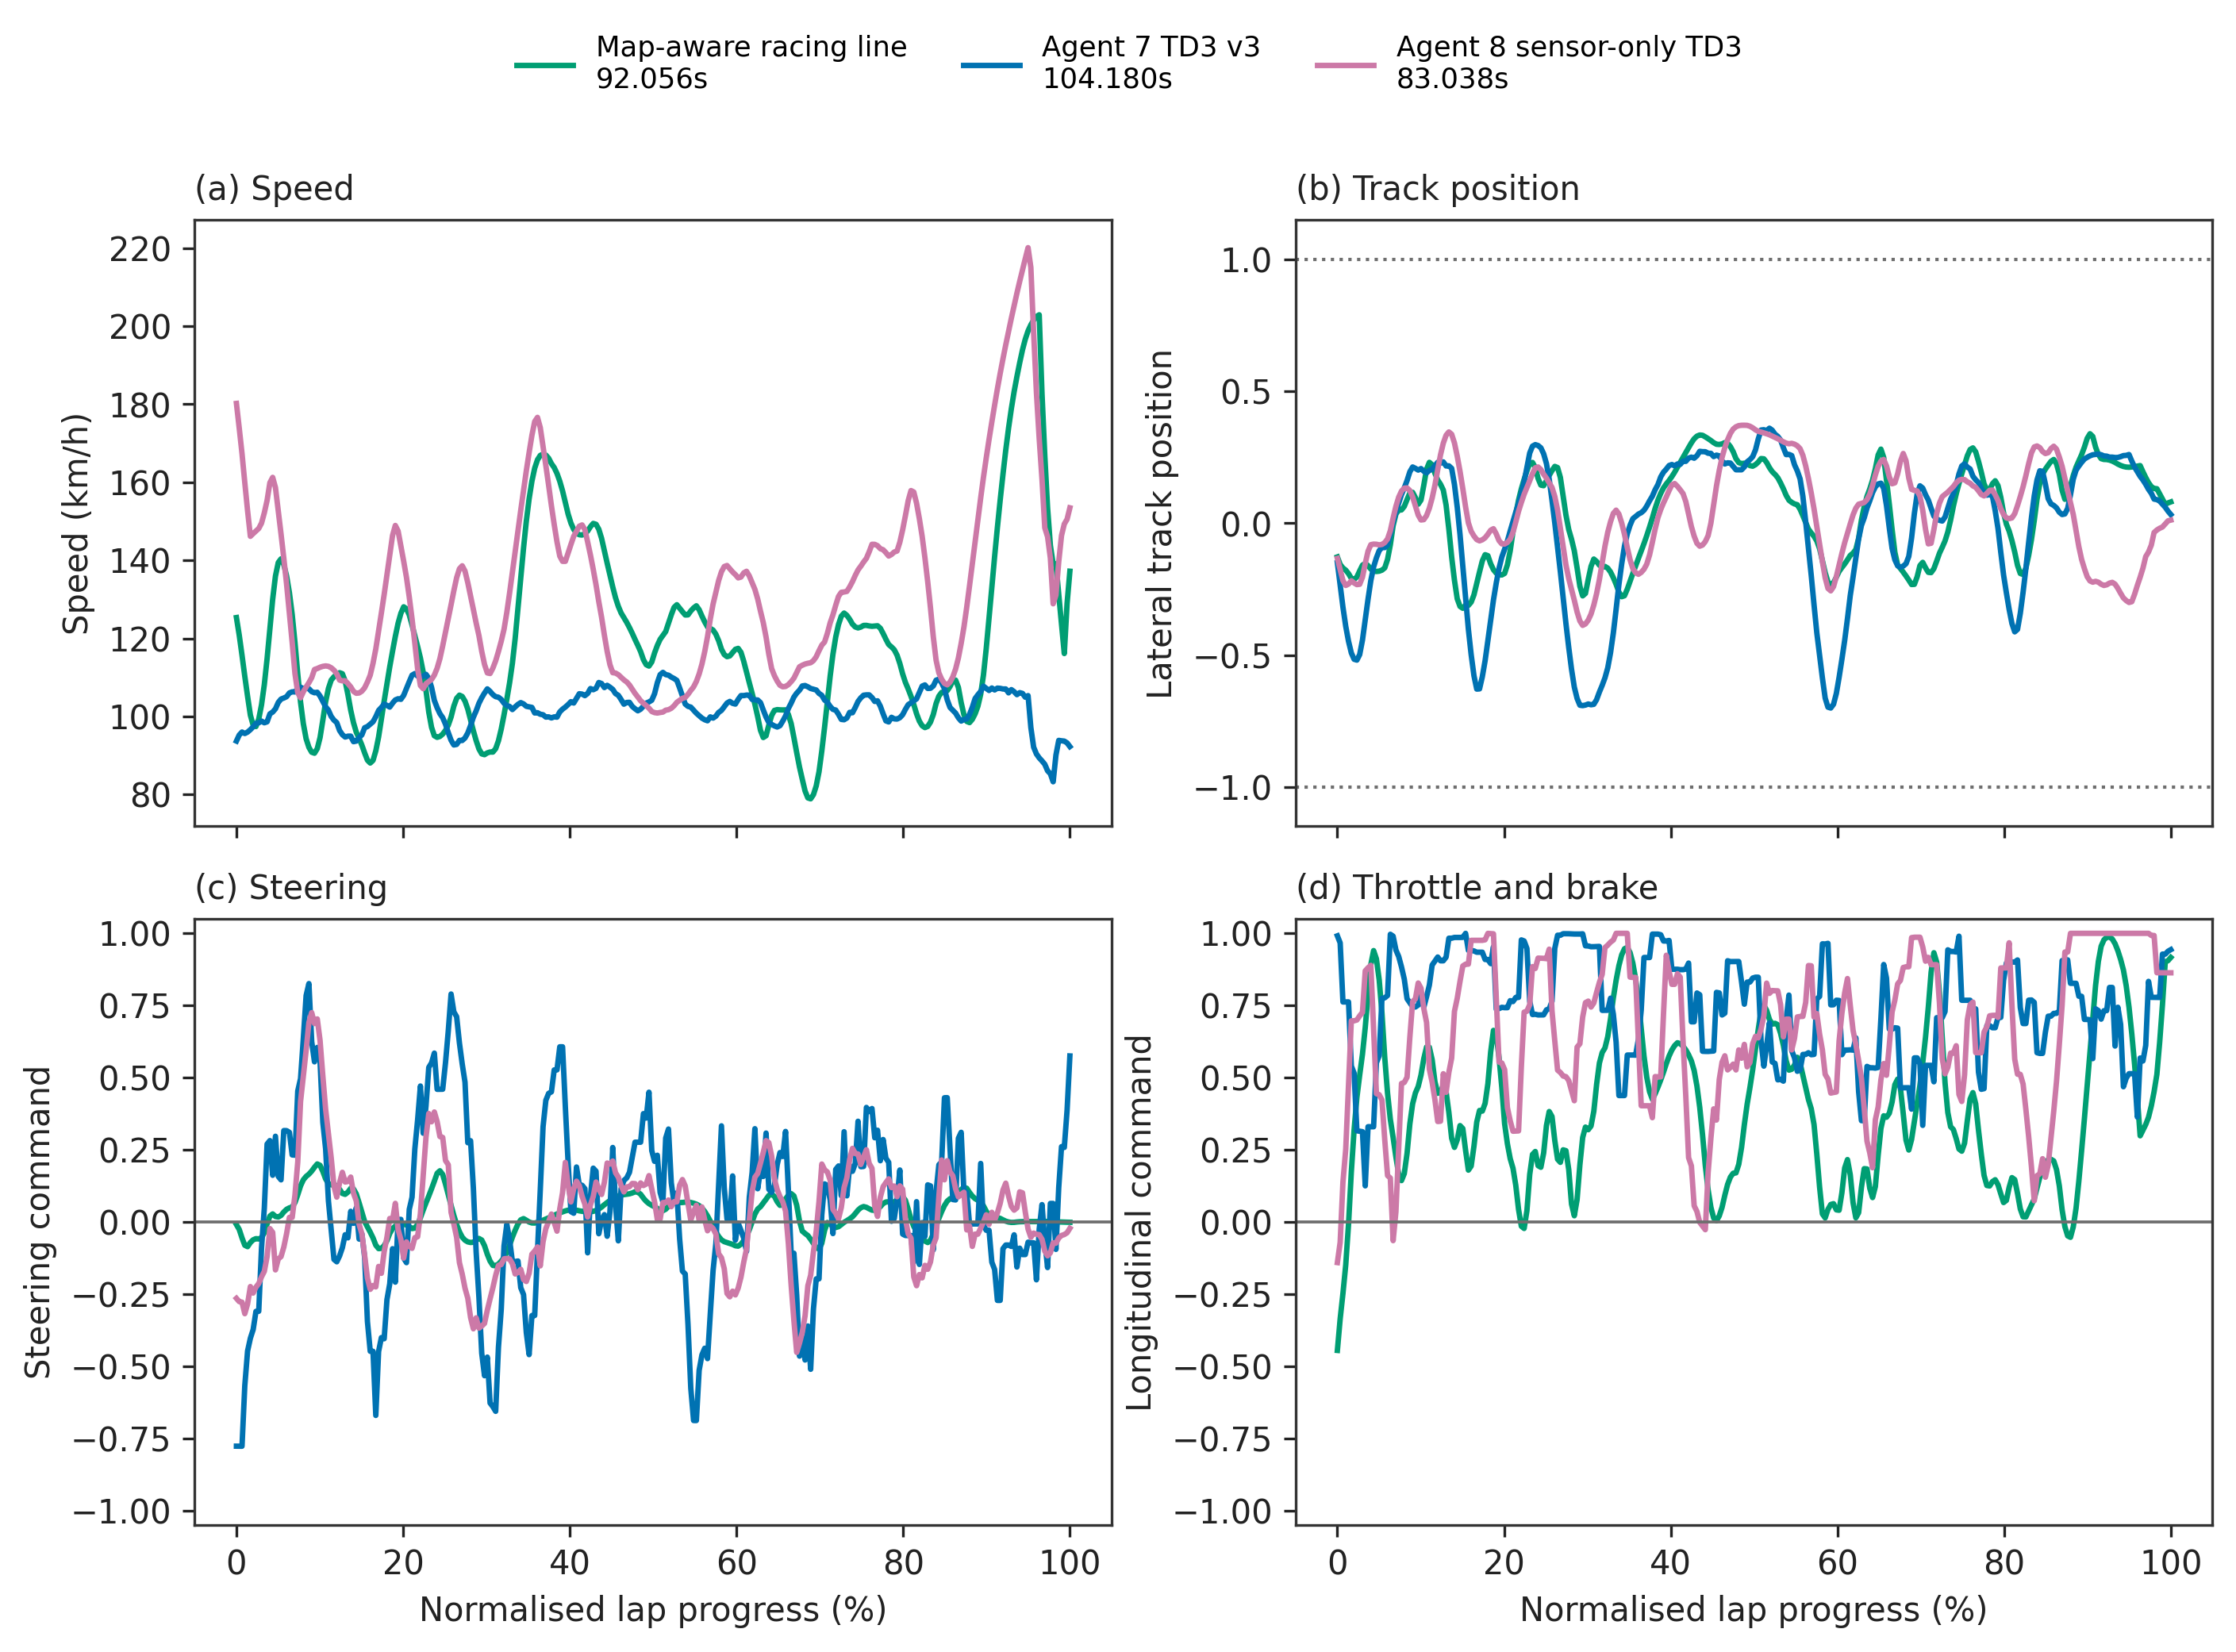
\includegraphics[width=\textwidth]{figure_10_5_control_profiles.png}
  \caption{Control profiles for representative completed laps. Speed, lateral position, steering and longitudinal action are aligned by normalised lap progress. The dotted lateral boundaries denote the track edge. Each line is a descriptive stored trace chosen near the relevant group median, resampled to a common grid and smoothed with a nine-point display window. Source: project telemetry records.}
  \label{fig:control-profiles}
\end{figure}

Agent~8 reaches higher speeds on several sections while remaining within the lateral boundaries in this trace. Agent~7 has larger steering reversals, consistent with its slower pace; the map-aware controller has a distinct longitudinal pattern because route and curvature are explicit. These profiles explain the stored outcomes but do not establish a causal ranking, since the policies differ in observation, reward and training history.

\subsection{Application result}

The evidence is not confined to scripts and model folders. The packaged application lets a user select an agent, start TORCS, inspect live telemetry, review a stored run and compare agents in one interface. Failure is informative rather than hidden: termination labels and telemetry distinguish stalling, reverse travel and leaving the circuit.

This supports the novice-facing objective: an AI newcomer can see why one fast lap is insufficient and compare rules, track information and learned policies without reading code. It is functional evidence of accessible deployment and explanation, not a claim of proven educational improvement.

\section{Discussion}
\label{ch:discussion}

\subsection{Interpreting the result, rather than selecting a winner}

The numerical results do not support a simple story in which increasingly sophisticated algorithms necessarily produce increasingly better drivers. The Rule-Based and Map-Aware agents completed their stored application runs reliably, while the Dyna-Q and scratch-TD3 stages did not. This progression is an important finding. It shows that autonomous racing success depends on the relationship between representation, control resolution, reward design and evaluation, rather than on attaching a reinforcement-learning label to a controller.

The Map-Aware Racing-Line Agent is consequently a substantive result, not merely a preliminary baseline surpassed by a neural policy. It combined 15 completions from 15 stored attempts with a 92.056-second median completed lap and no recorded off-track events. Its design makes lateral error, target path and curvature interpretable. Where the circuit is known and explanation is valuable, that transparency is a practical advantage. The cost is that performance relies on track-specific route information, precisely the limitation anticipated by planning-ahead research \parencite{quadflieg2010}.

Agent~8 achieved the strongest observed final learned result: 36 completions from 40 repeated attempts and an 83.038-second median completed lap. This evidence supports a carefully bounded claim: under the fixed \texttt{g-track-3} scenario and final deployment contract, a sensor-only N-step TD3 policy achieved the best observed balance of pace and repeated completion. It does not show that sensor-only learning is intrinsically superior to racing-line information, or that the policy would transfer to an unfamiliar circuit. Treating the result as conditional is not a weakness; it is the appropriate interpretation of one-track simulator evidence.

\subsection{What the Agent 7 and Agent 8 comparison means}

Agent~7 and Agent~8 were designed to make a meaningful question visible. Agent~7 receives racing-line geometry as context, whereas Agent~8 receives only vehicle and road-sensor observations plus short-term history. The success of Agent~8 shows that explicit route information was not necessary for a fast policy to emerge in this setting. It also makes the application more educational: users can compare a policy guided by an explicit target route with one that must infer a useful response from local sensor readings.

However, this comparison is not a controlled ablation of one variable. Agent~8's final policy differs from Agent~7 not only in geometry inputs but also in its reward and stability-focused training history. The self-imitation stage was a reasoned response to the early rare-fast-lap problem, but it remains a change to the training contract. The correct conclusion is therefore that the final implemented Agent~8 was stronger on the observed metrics, not that removing a racing line caused the improvement. A follow-up experiment should freeze the network, reward, training budget and checkpoint-selection rule, then vary only the geometry features.

This distinction is academically valuable. It identifies the next experiment that would convert an interesting applied comparison into a stronger causal claim. It also prevents the dissertation from overstating what its data show, a problem highlighted by deep-RL reproducibility research \parencite{henderson2018,agarwal2021}.

\subsection{Pace, reliability and evidence strength}

The results reinforce the decision to evaluate pace and reliability together. A 10/10 completion rate from Agent~7 v4 is encouraging, but it comes from a smaller batch than Agent~8's 36/40 result. Similarly, the Rule-Based agent's two completions demonstrate functional stability but are not a precise estimate of future reliability. The Map-Aware result has more evidential weight because it contains 15 attempts, while Agent~8's repeated 40-attempt evaluation provides the strongest final learned-policy evidence.

Median completed-lap time has a specific interpretation. It describes typical performance among laps that finished; it does not capture the cost of failed attempts. This is why Agent~8's 83.038-second median must always be read beside its 90\% completion rate, and why the Dyna-Q result cannot be described as merely \enquote{slow}. It was both slow when successful and unreliable across attempts. The GUI's decision to display trial count, completion percentage and termination information is therefore part of the research contribution, not a secondary presentation feature.

The use of two evidence streams is a further limitation and strength. Database records show that the deployed application can execute agents, store runs and make outcomes reviewable. Formal repeated evaluations more strongly support claims about fixed learned policies. These streams should not be collapsed into an unexplained aggregate, but neither should the database be dismissed: it verifies the end-to-end product behaviour required by the brief. Clear provenance allows the reader to assign appropriate weight to each result.

\subsection{The novice-facing contribution}

The application satisfies the core practical aim of the brief by reducing the work required before an AI newcomer can observe an agent. The complete release folder contains the executable, TORCS, policies and runtime data. The functional workflow is explicit: launch the package, select a named driver, observe its behaviour, review the stored outcome and compare its evidence with another agent. This removes cloning the repository, creating a virtual environment and locating a model checkpoint from the first encounter with the system. It is therefore a meaningful deployment and learning-design contribution, rather than a polished interface added after the experiment.

The interface also supports a more responsible explanation of machine learning. It does not present Agent~8 as a magic high score. It can show a learner that an agent may be fast but fail, that explicit rules can be stable, and that a racing line is a form of additional information rather than a guaranteed solution. This supports the initial AI-literacy aim described by \textcite{long2020}: users can connect an AI system's inputs, actions, capability and limitation to evidence from a visible task. It also aligns with human-AI interaction guidance that systems should communicate capability and limitation together \parencite{amershi2019}.

The limitation is equally clear. Functional accessibility is not the same as measured usability or learning. The project has shown that the workflow exists, that its acceptance conditions can be checked and that the packaged release can be smoke-tested, but it has not measured whether novice adults or students can correctly interpret a completion-rate comparison or explain the difference between the agents. A small task-based user study is therefore the most direct next step for validating the educational claim.

\subsection{Overall contribution and limitations}

The project contributes an integrated artefact rather than a single algorithmic score. It joins autonomous control, telemetry storage, evaluation provenance, visual explanation and novice deployment in one system. It also preserves unsuccessful learning stages, making the final Agent~8 result more credible because the path to it is visible rather than rewritten as a sequence of inevitable successes.

The remaining limitations bound the contribution. All primary evidence comes from one simulated circuit and one car. The final agents have unequal sample sizes and differ in more than one training variable. No formal user study has evaluated the explanatory interface. These constraints prevent claims of road-vehicle performance, general algorithmic superiority or proven educational impact. They do not negate the work; they define the appropriate scope of a well-evidenced MSc software and machine-learning dissertation.

\section{Conclusion and Future Work}
\label{ch:conclusion}

Enhanced AI Racing achieved its central aim: it delivered a TORCS application in which contrasting autonomous drivers can be run, evaluated and explained through a research-informed novice-facing learning platform. The project implemented a meaningful progression from random and rule-based behaviour to map-aware control, Dyna-Q and N-step TD3. It also reduced deployment friction through a Windows package that contains TORCS, runtime policies and the application launcher.

The results show that the map-aware controller is a strong transparent baseline, completing 15 of 15 stored application attempts with a 92.056-second median completed lap. Agent~8 delivered the strongest observed final learned result, completing 36 of 40 repeated evaluations with a median completed-lap time of 83.038 seconds. These findings support the value of continuous deep reinforcement learning for this configuration, while the weaker Dyna-Q and scratch-TD3 outcomes show why such a conclusion cannot be assumed in advance.

The work remains limited to simulated one-track evaluation and functional rather than participant-based novice assessment. Future work should evaluate all selected agents in equal-sized frozen-policy batches; run policies on unseen tracks; perform an ablation that isolates racing-line input from reward and training differences; quantify variation with appropriate intervals; and conduct a small novice usability study. These steps would extend the current project from a strong evidence-aware simulator artefact towards a broader study of robust autonomous control and AI education.

The final lesson is that the strongest system outcome combines performance with inspectability. The project would be less useful if the fastest policy could be started only through private scripts or its failures were hidden in a checkpoint directory. Conversely, a polished interface without a reliable evidence trail would not meet the standard of a research artefact. Enhanced AI Racing connects these concerns: it preserves the technical detail necessary for scrutiny while giving a beginner a workable route into observing and discussing autonomous decision-making.

Within its scope, the work therefore makes three defensible claims. It demonstrates that several autonomous-driving approaches can be integrated behind one TORCS application and assessed with common outcome semantics. It provides evidence that the final sensor-only TD3 policy achieved the strongest observed learned performance on \texttt{g-track-3}, while the map-aware controller remained a stable and interpretable engineered benchmark. Finally, it demonstrates a packaged, evidence-aware and research-informed learning platform through which an AI newcomer can launch, observe and critically compare those findings without development setup. These are substantial outcomes, provided their limits are retained: they are not claims of real-world vehicle autonomy, universal algorithmic superiority or verified educational impact.

\printbibliography[heading=bibintoc,title={References}]

\end{document}


